\documentclass[a4paper,10pt]{article}
\usepackage[utf8x]{inputenc}
\usepackage[margin=3cm]{geometry}
\usepackage{xspace,xcolor,amsmath,amssymb}
\usepackage{graphicx}
\usepackage[FIGTOPCAP,large,sf,bf,nooneline]{subfigure}
\usepackage{float,placeins,xspace}
\usepackage{authblk}
\usepackage{comment}

\renewcommand{\familydefault}{\sfdefault}

%opening
%\title{Quantifying self-maintained stability of protein patterns lacking external morphogen gradients}

\title{Stable developmental patterns of gene expression\\ without morphogen gradients}

\author[1]{Maciej Majka}
\author[2,3]{Nils B. Becker}
\author[2]{Pieter Rein ten Wolde}
\author[1]{Marcin Zagorski}
\author[2,4]{Thomas R. Sokolowski}

\affil[1]{Institute of Theoretical Physics and Mark Kac Center for Complex  Systems Research, Jagiellonian  University, ul. prof. Stanis\l{}awa   Lojasiewicza 11, 30-348 Krak\'{o}w, Poland}
\affil[2]{FOM Institute AMOLF, Science Park 104, 1098 XG Amsterdam, The Netherlands}
\affil[3]{Present address: Theoretical Systems Biology, German Cancer Research Center, 69120 Heidelberg, Germany}
\affil[4]{Present address: Frankfurt Institute for Advanced Studies (FIAS), Ruth-Moufang-Stra\ss{}e 1, 60348 Frankfurt am Main, Germany}


% NEW/CUSTOM MACROS
% redefine the subscript macro
\catcode`_=\active
\def_#1{\ensuremath{\sb{\mathrm{#1}}}}
% general
\newcommand{\TODO}[1]{\textcolor{blue}{\textbf{($\bigstar$ #1)}}}
\newcommand{\CITE}{\textbf{[C!]}\xspace}
\newcommand{\Drosophila}{{\it Drosophila}\xspace}
% gap gene names
\newcommand{\hb}{{\it hb}\xspace}
\newcommand{\kr}{{\it kr}\xspace}
\newcommand{\kni}{{\it kni}\xspace}
\newcommand{\gt}{{\it gt}\xspace}
\newcommand{\Hb}{{\it Hb}\xspace}
\newcommand{\Kr}{{\it Kr}\xspace}
\newcommand{\Kni}{{\it Kni}\xspace}
\newcommand{\Gt}{{\it Gt}\xspace}
\newcommand{\Bcd}{{\it Bcd}\xspace}
\newcommand{\Cad}{{\it Cad}\xspace}
\newcommand{\Tll}{{\it Tll}\xspace}
% generic gene names
\newcommand{\GA}{A\xspace}
\newcommand{\GB}{B\xspace}
\newcommand{\GC}{C\xspace}
\newcommand{\GD}{D\xspace}
% binding rates
\newcommand{\kRon}{k^{\rm R}_{on}}
\newcommand{\kRoffS}{k_{\rm s}^{\rm off}}
\newcommand{\kRoffW}{k_{\rm w}^{\rm off}}
\newcommand{\kDon}{k^{\rm D}_{on}}
\newcommand{\kDoff}{k^{\rm D}_{off}}
% further macros
\newcommand{\vecA}[1]{\vec{#1}}
\newcommand{\myvec}[1]{\overrightarrow{#1}}
\newcommand{\avg}[1]{\left\langle #1\right\rangle}
\newcommand{\unit}[1]{{\rm #1}}
\newcommand{\mum}{\unit{\mu m}}
\newcommand{\mumsps}{\unit{\mu m^2/s}}
\newcommand{\SI}{Supporting Text\xspace}
\newcommand{\mysubsubsection}[1]{\vspace{1EM}\noindent{\bf #1}\\}
%\newcommand{\MM}{``Methods'' section \ref{sec-GG-Methods}\xspace}
\newcommand{\MM}{``Materials and Methods''\xspace}
\newcommand{\myurl}[1]{\textsf{#1}} % TODO later replace by \url from hyperref
\newcommand{\mysubref}[1]{\normalfont (\subref{#1})}
\newcommand{\changed}[1]{{\color{red}#1}}



\hyphenation{Dro-so-phi-la me-la-no-gas-ter}
\hyphenation{Bi-coid}

\begin{document}
\def~{\nobreakspace{}}

\maketitle

\begin{abstract}
    Gene expression patterns are established by cross-regulating target genes that interpret morphogen gradients. However, as development progresses, morphogen activity is reduced, leaving the emergent pattern without stabilizing positional cues. The pattern then can be deteriorated by the intrinsically noisy biochemical processes acting at the cellular level. But remarkably, the established gene expression patterns remain spatially and temporally stable in many biological systems. Here we combine spatial-stochastic simulations with an enhanced sampling method (Non-Stationary Forward Flux Sampling) and a recently developed stability theory to address how spatiotemporal integrity of a gene expression pattern is maintained in developing tissue lacking morphogen gradients. Using a minimal embryo model consisting of spatially coupled biochemical reactor volumes, we study a stripe pattern in which weak cross-repression between nearest neighbor domians alternates with strong repression between next-nearest neighbor domains, inspired by the gap gene system in the {\it Drosophila} embryo. We find that fine-tuning of the weak repressive interactions to an optimal level can increase temporal stability of the expression patterns by orders of magnitude, allowing for stable patterns over developmentally relevant times in the absence of morphogen gradients. The numerically determined optimal parameter regime closely agrees with the predictions of the stability theory. By analizing the properties of the reduced phase space defined by pattern asymmetry factors that characterize pattern integrity, we trace back the pattern stability enhancement to the emergence of a metastable basin that protects intact patterns from rapid destruction in the optimal repression regime via restoring forces that counteract pattern perturbations. Altogether our results demonstrate that metastable attractors can emerge as a property of stochastic gene expression patterns even without system-wide positional cues, provided that the gene regulatory interactions shaping the pattern are optimally tuned.
\end{abstract}

\clearpage 

\section{Introduction}
%%The temporal maintenance of stable and precise protein patterns is crucial in many biological problems.Perhaps the best studied example is early embryo development, where locally expressed morphogenetic patterns determine divergent cell fates and thus initiate distinct development of different body parts. \TODO{refs}Such patterning mechanisms are implemented by gene regulatory networks, which are inherently noisy;it is therefore unclear how stable patterns can be maintained by such mechanisms over longer times.

%The temporal maintenance of stable and precise protein patterns is crucial in many biological problems.
Maintaining the integrity of spatial gene expression patterns over time is essential in embryonic development. In early embryo development locally expressed morphogenetic proteins spread through the tissue to form gradients of chemical signals \cite{Gregor2007a,Rogers2011,Lander2011,Balaskas2012,Kicheva2012,Shvartsman2012,Briscoe2015,Bier2015,Stapornwongkul2020,Stapornwongkul2021,Simsek2022}. Inside developing cells, these chemical signals are interpreted by gene regulatory networks to form remarkably precise and reproducible spatial patterns of gene expression that subsequently give raise to different body parts and organs \cite{Gregor2007b,DubuisPNAS2011,Sokolowski2012,Wu2015,Zagorski2017,Petkova2019,Kuzmicz-Kowalska2020,Tkacik2021,Exelby2021,Iyer2022,Sokolowski2023,Minchington2023}. However, as spatial patterns are established by reading out upstream morphogen gradients, their stability is constantly subject to inherently noisy cellular and extracellular processes \cite{Swain2002,Raser2005,Paulsson2005,Raj2008,Chalancon2012,Averbukh2017}. 
Moreover, the activity of morphogenetic gradients that is interpreted by target cells can decrease over developmental time. This decrease in activity can take different forms, including reduction of the relative signaling range as the embryo grows in size \cite{Zagorski2017,Kicheva2014}, signalling pathway desensitization \cite{Cohen2015}, or complete disappearance of the gradients at later developmental stages \cite{Drocco2011,Durrieu2018}. Together, the inherent cellular stochasticity and reduced role of morphogen gradients at later stages raise the question about how stable patterns can be maintained over sufficiently long developmental times.
%%%I suggest to start new paragraph here, possibly extend the previous one by one or two sentences in the middle%%%

Focusing on the cellular stochasticity, biological cells are facing two types of noise, namely intrinsic and extrinsic noise, with different notions of robustness against the respective noise types \cite{Swain2002,Raser2005,Paulsson2005,Raj2008,Chalancon2012,Averbukh2017}. Intrinsic noise originates from the processes of gene regulation, protein production, and intracellular transport. Thus,  robustness of spatial patterns to intrinsic noise amounts to buffering random fluctuations in the copy numbers of patterning proteins. Extrinsic noise, on the other hand, terms the variations originating from different external conditions including cell size variability \cite{Huh2011,Thomas2019}, cell-to-cell variation in ribosome abundance \cite{Raj2008} or fluctuations in the cellular environment \cite{Pedraza2005,Stockholm2010}. Therefore, the robustness of spatial patterns to extrinsic noise refers to the capability of producing precise patterns in spite of imperfect initial conditions, classically termed ``canalization'' in Waddington's picture of development \cite{Waddington1942,Waddington1959}. Several gene regulatory strategies providing either type of robustness have been studied \cite{Simsek2022,Iyer2022,Averbukh2017}, but our understanding of how nature orchestrates them in the fully interacting wild-type organism is still incomplete.

%Intriguingly, one regulatory motif commonly occurring in many patterning systems is mutual repression \cite{Alon2007,Vakulenko2009,Cotterell2010,Burda2011,Sokolowski2012,Balaskas2012,Zagorski2017,Verd2017,Verd2019}. It is thus natural to ask whether and how this network motif aids enhancing pattern robustness. Importantly, since mutual repression itself can induce bistability and associated stochastic switching, it is a priori unclear whether it constitutes a benefit or further detriment to pattern stability. This issue is particularly pertinent to systems that lack any external cues for symmetry breaking, such as maternal gradients, that could force the bistable cells into one of their opposing fates. 

Among the regulatory mechanisms that drive developmental pattern formation, the regulatory motif in which two genes mutually repress each other is particularly prevalent \cite{Balaskas2012,Alon2007,Vakulenko2009,Cotterell2010,Burda2011,Martin2016,Verd2017,Verd2019,Exelby2021}. Intriguingly, mutual repression can have a dual role in the establishment of spatial patterns. On the one hand, in systems driven by threshold-dependent activation of patterning genes via morphogen gradients, mutual repression is crucial for shaping out expression domains that are bounded from two sides, thus increasing the positional information carried by the expression pattern \cite{Sokolowski2012,Sokolowski2015,Zagorski2017,Exelby2021,Sokolowski2023}. On the other hand, mutual repression can induce bistability leading to stochastic switching between cell fates. Hence, it is a priori unclear to which extent mutual repression supports or counter-acts the formation of stable spatial patterns \cite{Sokolowski2012,Zagorski2017,Exelby2021}. This issue is particularly relevant to systems that lack external cues for symmetry breaking, such as morphogen or maternal gradients, that could force bistable cells into one of their opposing fates.

Here we ask whether a system of mutually interacting genes can maintain an initially arranged expression pattern in the absence of upstream input gradients. To address this question we study a spatially resolved gene regulatory network, conceptually motivated by the gap gene system in the early embryo of the fruit fly {\it Drosophila melanogaster} \cite{Jaeger2004, Jaeger2011, Dubuis2013, Manu2009PlosBiol, Surkova2008, Clyde2003}.
This system implements a particular regulatory architecture, 
in which weak and strong mutual repressive interactions between expression domains of different genes alternate depending on whether the domains are adjacent or not.
%This motif was termed ``alternating cushions'' and found to entail robustness to extrinsic noise in earlier theoretical work \cite{Vakulenko2009}; specifically, that work, using a deterministic model, established the existence of repulsing forces between the expression domains (``cushions'').
This motif, termed ``alternating cushions'', was earlier investigated in terms of stability and robustness against extrinsic noise in initial conditions \cite{Vakulenko2009}. That study employed a reaction-diffusion model with step-like activation functions for representing the underlying gene expression dynamics. Using the so-called ``moving kink approximation'', the study predicted an extensive basin of pattern stability in the parameter space of the model, where the stability could be attributed to repulsive forces between mutually repressing gene expression domains (``cushions''). More recently, an exact solution was obtained in an analogous model for the dynamics of the contact zones between two gene expression domains and for arbitrary combination of activating or repressing interactions between the involved genes \cite{Majka2023}. This work provided exact stability conditions, leading to a better quantitative understanding of the conditions under which stochastically driven gene expression patterns can remain stable. Importantly, it was shown that perfect pattern stability (i.e., a pattern surviving for arbitrarily long time) can only be achieved for a very specific combination of system parameters; nevertheless, in the vicinity of these states, there exists a continuity of well-defined but slowly travelling gene expression patterns, which can fulfill their biological role for a finite but in many cases sufficiently long period of time. However, it remained unclear whether the derived stability conditions also remain valid under genuinely stochastic conditions.

% In order to test this new theory and investigate whether the deterministic reaction-diffusion model of pattern stability can be succesfully applied to the, ultimately, stochastic gene expression dynamics, 
Here we assess the temporal stability of gene expression patterns interacting via the ``alternating cushions'' motif by numerical simulations of a minimal spatial-stochastic model that features a full microscopic representation of stochastic gene expression and protein diffusion, thus incorporating the relevant intrinsic noise sources.
%In order to investigate comprehensively the robustness of this motif to both extrinsic and intrinsic fluctations, we first simulate a minimal spatial model system that features a full microscopic representation of stochastic gene expression and protein diffusion, thus incorporating the relevant intrinsic noise sources.
Using Non-Stationary Forward Flux Sampling (NS-FFS) \cite{BeckerTenWolde2012,BeckerAllenTenWolde2012}, an enhanced biased sampling technique for stochastic systems changing in time, we quantify for how long patterns shaped and maintained only by mutual repression can self-maintain themselves. Moreover, we expand the stability theory from \cite{Majka2023} to the case of multiple interfaces and identify the parameter regime within which boundaries between adjacent gene expression domains are predicted to remain stable.
%In addition, based on our earlier work \cite{Majka2023}, we derive and solve a mathematical representation of the simulated model and identify the parameter regime within which boundaries between adjacent gene expression domains are predicted to remain stable.

% We find that the staggered regulatory architecture can drastically enhance the pattern stability and 
% maximize its self-maintenance time when the strength of mutual repression is fine-tuned.
% This can be traced back to the presence of a dynamical attractor / metastable basin in the underlying phase space.

Our results show that the stability of patterns arranged in the alternating cushions scheme strongly varies with the strength of mutual repression between adjacent gene expression domains. 
We find that pattern stability time is maximized when spatially adjacent genes repress each other with intermediate strength while the next-nearest neighbor genes repress each other strongly. 
In this optimal regime, we confirm the existence of robust restoring forces and find signatures of a metastable basin that stabilizes well-ordered patterns (dynamical attractor), in accordance with the previous findings of \cite{Vakulenko2009}.
Away from the optimum, forces induced by strong nearest neighbor mutual repression destroy the stripe patterns rapidly, while for weaker nearest neighbor repression the forces are imperceptible when compared to stochastic fluctuations. At the same time, the numerically determined optimal parameter regime is situated in the vicinity of the theoretically predicted optimum. While the adapted theory indicates a single optimal choice of parameters ensuring a perfectly stable pattern, the simulations uncover a parameter range over which pattern stability is enhanced but always finite.% On the methodological level, this also shows that it is possible to map a complex microscopic model on the effective equations of expression dynamics. Then, using the stability theory for this effective model, one can find the approximated value of optimal parameters, which can significantly reduce the computational load of numerical search.
%The optimal regime found via NS-FFS-driven simulations agrees with the stability regime predicted by our mathematical theory.

Taken together, we demonstrate that forces generated in the alternating cushions scheme can maintain the gene expression pattern subject to stochastic production and diffusion of proteins for extremely long times if the parameters of mutual repression are optimized.

\mysubsubsection{Modelling framework}

In order to investigate stability of gene expression patterns without external input gradients, we performed stochastic simulations of a spatial pattern of four mutually repressing genes, using NS-FFS.
%While developmental patterns can be astonishingly precise and reproducible \cite{Houchmandzadeh2002, Gregor2007a, Gregor2007b, Petkova2019, Tkacik2021}, the processes that drive it, in particular gene expression, are very stochastic.
%It is therefore natural to ask for the mechanisms that attenuate gene expression noise in development.
%such as spatial averaging \cite{Erdmann2009} and mutual regulatory interactions \cite{Sokolowski2012, Manu2009PlosBiol},
%Addressing this question requires a spatially resolved stochastic model.
Here we opted for a minimal spatially resolved stochastic model, shown in schematic Fig. \ref{Fig-ModelSketch}, inspired by the the posterior gap gene pattern in \Drosophila development \cite{Jaeger2004}. The model considers four mutually interacting genes \GA, \GB, \GC and \GD, arranged in a five-stripe pattern (with order \GA-\GB-\GC-\GD-\GA) along a cylindrical spatial lattice. The four genes are analogous to the arrangement of the expression domains 
of gap genes \hb, \kr, \kni and \gt in nuclear cycle 14 in the posterior half of the early fly embryo, where \hb is expressed in two domains, in the first (anteriormost) and last (posteriormost) expression domain \cite{Jaeger2004, Jaeger2011, Dubuis2013, Manu2009PlosBiol, Surkova2008, Clyde2003}.
The spatial lattice consists of $N_z\times N_\phi$ equally spaced and well-stirred reaction volumes with periodic boundary conditions in the circumferential ($\phi$-) direction motivated by the arrangement of cortical nuclei in the developing fly embryo.
Protein diffusion and nuclear exchange are modeled via hopping between neighboring reaction volumes, with a rate proportional to the diffusion coefficient.
% To account for the radial symmetry of the embryo 
% we impose periodic boundary conditions in the circumferential lattice direction,
% which enables diffusive hopping from lattice site $(z,N_\phi)$ to lattice site $(z,1)$, and vice versa
% (here $z$ and $\phi$ denote lattice indices in the axial and circumferential direction, respectively).
In each nucleus, proteins of the genes \GA, \GB, \GC and \GD are produced from their corresponding promoters, dimerize and mutually repress each other by promoter binding.
Each gene can repress the promoter of each other gene. %However, the repression strength differs among different gene pairs, as discussed further below.
Repression is non-competitive, i.e., each promoter has binding sites for each of the three other genes' dimers and is inactivated when at least one dimer is bound (``OR''-logics).
The model combines transcription and translation into one production step, neglecting some features of eukaryotic gene expression such as transcriptional bursts and enhancer dynamics, but previous work has shown that this does not alter the results qualitatively \cite{Erdmann2009,Sokolowski2012}.

%%%%%%%%%%%%%%%%
%%% FIGURE 1 %%%
%%%%%%%%%%%%%%%%
\begin{figure}[ht!]
  %\listoffigures
  \centering
  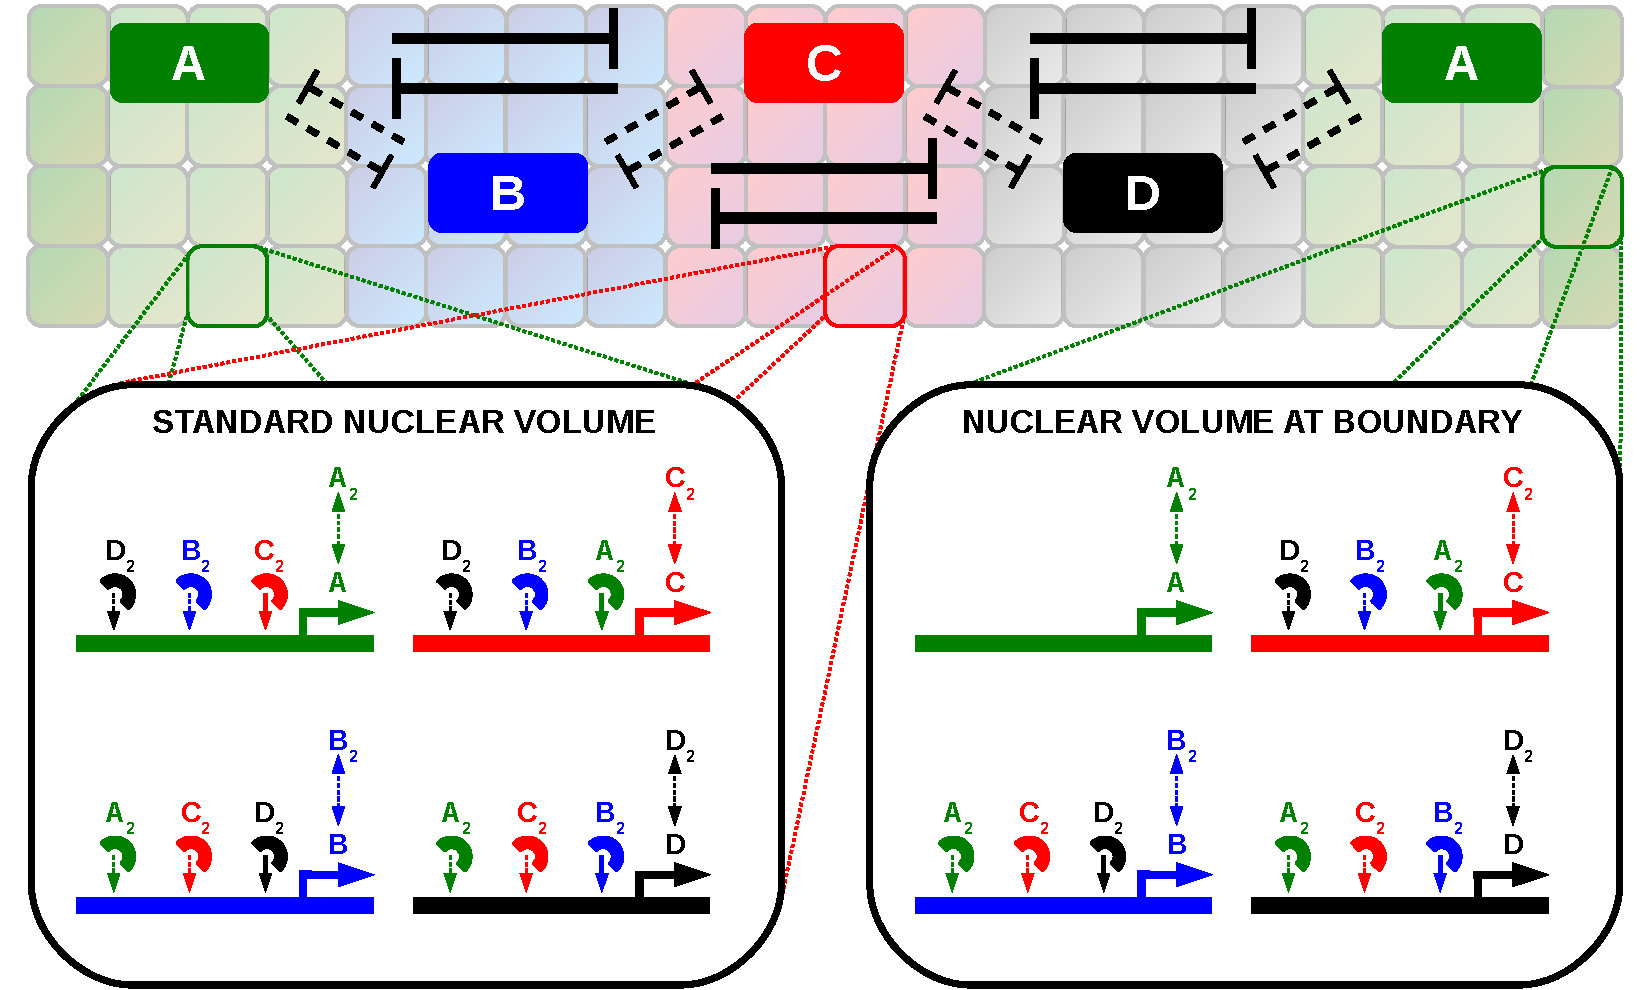
\includegraphics[width=0.9\textwidth]{Figures/FigureModel.pdf}
  \caption{\textbf{Schematic of the spatial gene-regulatory model.}
      We use a cylindrical lattice of reaction volumes
      to mimic the arrangement of cortical nuclei in the posterior \Drosophila embryo at developmental cycle 14.
      In each nuclear volume (shaded squares) we simulate production, degradation, dimerization and mutual repression of the four genes \GA, \GB, \GC and \GD via the Gillsepie algorithm.
      Each gene is subject to repression by the protein dimers of the other genes,
      as indicated by the schematic promoters. Neighboring nuclei can exchange monomers and dimers via diffusive hopping. The system is initialized in a five-stripe pattern of expression domains in the order \GA--\GB--\GC--\GD--\GA, corresponding to the experimentally observed order in the fly embryo.
      The strength of mutual repression varies among gap gene pairs: genes associated with nearest neighbor (NN) domains repress each other weakly (dashed arrows), while next-nearest neighbors (NNN) domains exhibit strong mutual repression (thick arrows).
      By default, the concentration of \GA is pinned at the system boundary where
      the set of modelled reactions differs from the rest of the system by the fact that
      the \GA promoter can not be repressed.
      %Note that this deliberately simplifying drawing does not depict the cylindrical model geometry in all details; 
      Details in the Methods, Sec. \ref{sec-GG-Methods}.
  \label{Fig-ModelSketch}
  }
\end{figure}

In the anterior-posterior arrangement \GA-\GB-\GC-\GD-\GA, the genes repress each other mutually via the characteristic pattern of strong next-nearest neighbor (NNN) and weaker nearest-neighbor (NN) repression (alternating cushions), as observed in the \Drosophila embryo \cite{Vakulenko2009, Jaeger2004, Clyde2003, Kraut1991a, Kraut1991b, Eldon1991, Hulskamp1990, Jackle1986}.
Specifically, there are two pairs of strongly repressing genes, (\GA,\GC) and (\GB,\GD), and four pairs of genes that repress each other weakly, (\GA,\GB), (\GB,\GC), (\GC,\GD) and (\GD,\GA).
In our model, the difference in repression strength is tuned via the unbinding rate of the repressors from the repressed promoter.
The strong-repressor unbinding rate $\kRoffS$ is chosen such that the NNN pairs (\GA,\GC) and (\GB,\GD) are in the bistable regime, while the weak-repressor unbidning rate $\kRoffW$ is varied. In this context, bistability corresponds to only one of the two competing genes being expressed at the single-nucleus level.
In the absence of cues capable of forcing the bistable systems into a preferred state, stochastic switching is expected to eventually result in one of the domains to dominate over the respective other domain in the NNN pair, causing its elimination and simultaneous expansion of the dominating gene's domain. This partial breakdown of the initial pattern can happen independently for both strongly repressing NNN pairs and thus in random temporal order; however, ultimately one of the strong repression partners is eliminated in each of the NNN pairs and the system settles in a new, effectively irreversible state in which only the remaining two genes are co-expressed.

On the one hand, we expect that the presence of the third expression domain in between the NNN pair domains can impede elimination of (one of) the NNN pair domains when NN repression is present.
On the other hand, overly strong NN repression is expected to enhance pattern breakdown because then even the overlapping NN expression domains are brought towards the bistable regime.
We therefore study the pattern stability as a function of the \emph{repression strength ratio} $\kappa$, defined as
\begin{align}
 \kappa \equiv \kRoffW / \kRoffS	\;,
 \label{Eq-kappa}
\end{align}
where $\kRoffW$ and $\kRoffS$ are the repressor unbinding rates for weakly repressing NN pairs and strongly repressing NNN pairs, respectively. $\kappa$ is varied through the weak repression unbinding rate $\kRoffW$. For $\kappa = 1$, i.e. $\kRoffW = \kRoffS$, both the NNN and the NN gene pairs are deeply in the bistable regime, while in the opposite limit $\kappa \rightarrow \infty$ ($\kRoffW \rightarrow \infty$) the NN pairs do not affect each other at all.


%\newpage
\section{Results}



%Figure \ref{Fig-TypicalOutput} shows typical simulated patterning protein profiles of an intact, relaxed pattern.

\mysubsubsection{Pattern stability is quantified by asymmetry factors}

A typical spatial pattern of gene expression with equally-sized domains is shown in Fig. \ref{Fig-TypicalOutput}.
In order, to quantify pattern stability we measure, as a function of $\kappa$, the average time until at least one domain is lost.
Further, in our system the strong NNN repression effectively prohibits coexistence of the strongly repressing genes at one location. Hence, the increase in size of one domain is always accompanied by a reduction in of the domain with its strong interaction partner. %\pagebreak
This lead us to introduce the following two order parameters, $\lambda_{AC}$ and $\lambda_{BD}$, here termed {\it asymmetry factors}, that measure the asymmetry for each of the two strongly antagonistic NNN pairs:
% and track progress towards pattern with at least one domain lost:
\begin{align}
 \lambda_{AC} \equiv \max([\GA]_{tot},[\GC]_{tot}) / N	\,, \qquad
 \lambda_{BD} \equiv \max([\GB]_{tot}, [\GD]_{tot}) / N	\,. \label{eq:lambdaACBD}
\end{align}
Here $[P]_{tot}$ is the \emph{total} copy number of P proteins (counting dimers twice), and $N=[\GA]_{tot} + [\GB]_{tot} + [\GC]_{tot} + [\GD]_{tot}$ is the total protein number in the system across all species.
In the spatially well-ordered pattern each protein domain occupies roughly the same fraction of the system, such that $\lambda_{AC} \simeq \lambda_{BD} \simeq 0.25$.
As expansion of a domain progresses at the expense of its strong antagonist, $\lambda_{AC}$ (or $\lambda_{BD})$ is enlarged and reaches values around $0.5$ when the shrinking domain is eventually lost.
In order to track progress of complete pattern losing one of its domains, we use sum $\lambda = \lambda_{AC} + \lambda_{BD}$, with values around $0.5$ for five-stripe patterns and values above $0.75$ indicating pattern breakdown.
%In short, $\lambda$ measures increasing asymmetry between strong repression partners as the system proceeds towards collapse.

%%%%%%%%%%%%%%%%
%%% FIGURE 2 %%%
%%%%%%%%%%%%%%%%
\begin{figure}[ht!]
  %\listoffigures
  \centering
  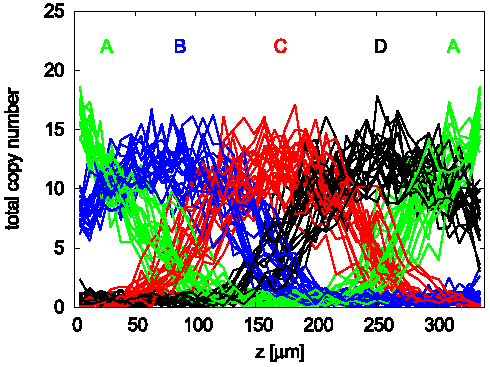
\includegraphics[width=0.6\textwidth]{Figures/FigureSystemDynamicsPinnedStable.pdf}
  \caption{\textbf{Spatial pattern of gene expression.}
      Snapshots of the total copy numbers of all considered patterning proteins
      as a function of the axial coordinate $z$ of the cylinder, averaged over its circumference.
      Colors correspond to Fig. \ref{Fig-ModelSketch} (green = \GA, blue = \GB, red = \GC, black = \GD).
      Snapshots were taken every $60~\unit{min}$ over a total simulated time of $20~\unit{h}$ after
      an initial relaxation phase of $30~\unit{min}$, starting from rectangular domain profiles
      of equal length. No-flux boundary condition at either end.
  \label{Fig-TypicalOutput}
  }
\end{figure} 

Our initial simulations revealed that even for very low protein copy numbers ($\lesssim 20$) the waiting times until one domain is lost are long compared to the duration of the actual breakdown event, and therefore difficult to sample by direct simulation. This lead us to ask, whether the five-stripe pattern is stabilized by a potential barrier that separates it from the pattern with fewer domains. Alternatively, the five-stripe pattern might not be stabilized by a potential barrier, but by a kinetic effect, where progress towards pattern breakdown is a slow directed process.
%resulting in its slow, but irreversible progress towards losing one of the domains.
%We thus cannot assume a priori that pattern destruction is an activated barrier-crossing process.
%This means that to investigate pattern breakdown, the full history of the trajectories has to be taken into account; we cannot presuppose rapid equilibration within the basin of the initial state.
In order to resolve which of these alternative mechanisms is responsible for the stabilization of the expression pattern, we combined our stochastic simulations with Non-Stationary Forward Flux Sampling (NS-FFS), which is particularly suited for enhanced sampling of non-equilibrium rare events. %we resorted to NS-FFS, which is suited for handling non-equilibrium systems with transient rare events.
We used $\lambda$ as the progress coordinate for NS-FFS, which aims at generating a branched and weighted trajectory ensemble that, in the most favorable cases, samples the relevant $\lambda$-range uniformly. This allowed us to generate sufficient statistics of rare breakdown events even in the most stable regions of parameter space (see Methods, Sec. \ref{sec-GG-Methods}) .
%Details of the setup are described in ``Methods'' section \ref{sec-GG-Methods}.

The early simulations also showed that the expression domains of gene \GA at the boundaries of the system (green expression domains in Fig.~\ref{Fig-TypicalOutput}) are particularly prone to destruction by their opponent domains, because they can only expand into one direction, towards the interior of the system.
We therefore decided to keep constant the level of \GA proteins in the volume at the system boundaries by locally disallowing repression in the outermost nuclei at the boundaries.
%this is motivated by the fact that in the \Drosophila gap gene pattern \Hb, the gene corresponding to \GA in our system, is in excess and under stringent control by \Bcd \cite{Driever1989}, 
%whereas in the posterior \hb expression is driven by a second enhancer under the control of \Tll \cite{Margolis1995},
%which in turn is directly controlled by the maternal terminal system and thus tightly localized \cite{Casanova1990, Weigel1990}.
To assess how this model assumption influences our results, we later compare to simulations in which \GA could vary at the system boundaries, finding that our main findings also hold in this less restricted system.

%Further model details are given in the ``Methods'' section \ref{sec-GG-Methods}.

%%%%%%%%%%%%%%%%
%%% FIGURE 3 %%%
%%%%%%%%%%%%%%%%
\begin{figure}[ht!]  
  \centering
  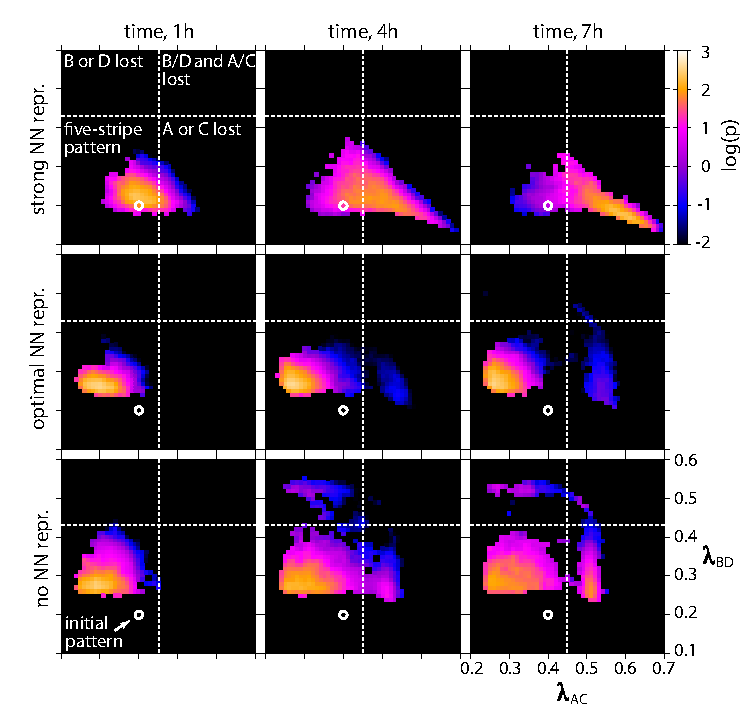
\includegraphics[width=\textwidth]{Figures/FigurePhaseSpaceComicV5.pdf}
  \caption{\textbf{Pattern breakdown in the phase space spanned by asymmetry factors.}
      Probability density snapshots of the phase space spanned by asymmetry factors $\lambda_{AC}$ and $\lambda_{BC}$, defined in \eqref{eq:lambdaACBD}, 
      at different times $t$ for varied repression strength ratio $\kappa$. The conditions are following: strong NN repression, $\kappa=3.16$ (top row), optimal NN repression for pattern stability, $\kappa=31.6$ (middle row), and lack of NN repression, $\kappa=\infty$ (bottom row). The simulation was started with the initial rectangular five-stripe \GA-\GB-\GC-\GD-\GA pattern $(\lambda_{AC}, \lambda_{BD})$=$(0.4,0.2)$ (white circle) in the pinned system. All snapshots are normalized histograms of reweighted $(\lambda_{AC}, \lambda_{BD})$-points within $t\pm5~\unit{min}$.
      In the middle and bottom rows we identify three densely populated regions:
      a broad region centered around $(0.30,0.30)$, $R_S$, which contains five-stripe patterns,
      and two smaller regions close to $(0.55, 0.30)$, $R^\dagger_{AC}$, and $(0.30, 0.55)$, $R^\dagger_{BD}$,
      representing patterns with one domain lost (region boundaries (dashed white), details in Methods,  Sec. \ref{sec-GG-Methods}). Ultimately trajectories will converge towards region centered around $(0.55, 0.55)$, $R^\ddagger$, where two domains are lost. %Note the two different pathways to destruction, of which the one via $R^\dagger_{AC}$ is preferred over the one via $R^\dagger_{BD}$. [this should go somewhere in the main text]
  \label{Fig-DensityPinned}
  }
\end{figure}


%\mysubsubsection{Metastable expression patterns are maintained for much longer times when the repression strength is optimal}
\mysubsubsection{Long-term pattern stability requires optimal repression strengths}

\noindent In order to see how varied repression strength affects pattern stability, we reweighted histograms of simulated trajectories over the reduced phase space spanned by order parameters $\lambda_{AC}$ and $\lambda_{BD}$ at different times, for different values of $\kappa$ ranging from strong NN repression ($\kappa\simeq 3$) to the limit of non-interacting nearest neighbors ($\kappa=\infty$), see Fig. \ref{Fig-DensityPinned}. We found that there exists a region of stable expression patterns in phase space which is populated rapidly and then remains quasi-stationary, indicating that the system can remain in a metastable state if NN repression is moderate. In particular, the velocity with which the system escapes from the quasi-stationary region strongly depends on $\kappa$, with low and very high $\kappa$ resulting in quick pattern deterioration, and intermediate $\kappa$ values resulting in the most long-lived quasi-stationary states.

Stochastic fluctuations can lead to two different events corresponding to partial pattern destruction:
%differing by the sequence in which NNN genes accomplish to eliminate their respective strong antagonist.
one in which either the \GA or \GC domain is lost first and one in which either the \GB or \GD domain is lost first. Motivated by these observations we defined a region of stable patterns in terms of the asymmetry factors as $R_S \equiv \{(\lambda_{AC}, \lambda_{BD}) \arrowvert \lambda_{AC} \leq 0.45 \text{ and } \lambda_{BD} \leq 0.43 \}$, see Fig.~\ref{Fig-DensityPinned}. States that lie outside of $R_S$ are considered deteriorated patterns, and accordingly we also defined two regions $R^\dagger_{AC}$ and $R^\dagger_{BD}$ and a region $R^\ddagger$ accumulating patterns with one expression domain lost and patterns with two domains lost, respectively. The pattern survival probability $S(t)=\iint_{R_S} p(\lambda_{AC}, \lambda_{BD},t) d\lambda_{AC}d\lambda_{BD}$ is the probability for the system to remain in the region of stable patterns until time $t$. We have never observed re-entry into $R_S$. We found that $S(t)$ is well-described by an exponential decay, $S(t)\propto e^{-k_D t}$, for times $t$ larger than a certain lag-time $t_{lag}$. $k_D$ then defines a deterioration rate, corresponding to average pattern stability time or alternatively mean time until pattern has lost one of its domains,  $\tau_D \equiv 1/k_D$ (see Methods, Sec. \ref{sec-GG-Methods}).

%%%%%%%%%%%%%%%%
%%% FIGURE 4 %%%
%%%%%%%%%%%%%%%%
\begin{figure}[ht!]
  \centering
%   \subfigure[][]{
%     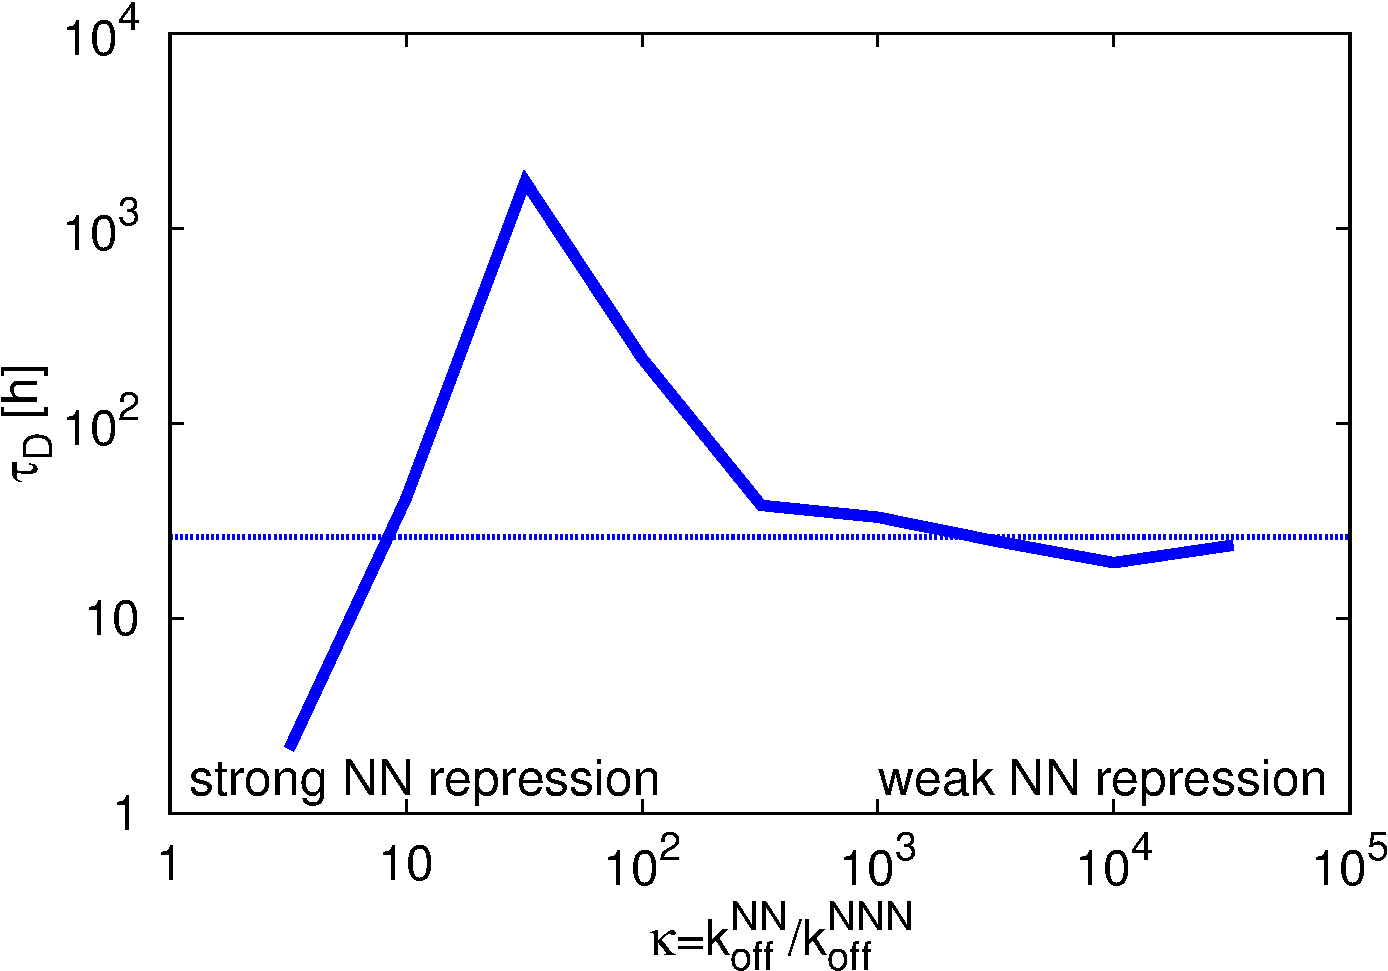
\includegraphics[width=0.66\textwidth]{Figures/FigureStabilityPinned.pdf}
%     \label{Fig-StabilityGrouped}
%   }\\
%   \subfigure[][]{
%     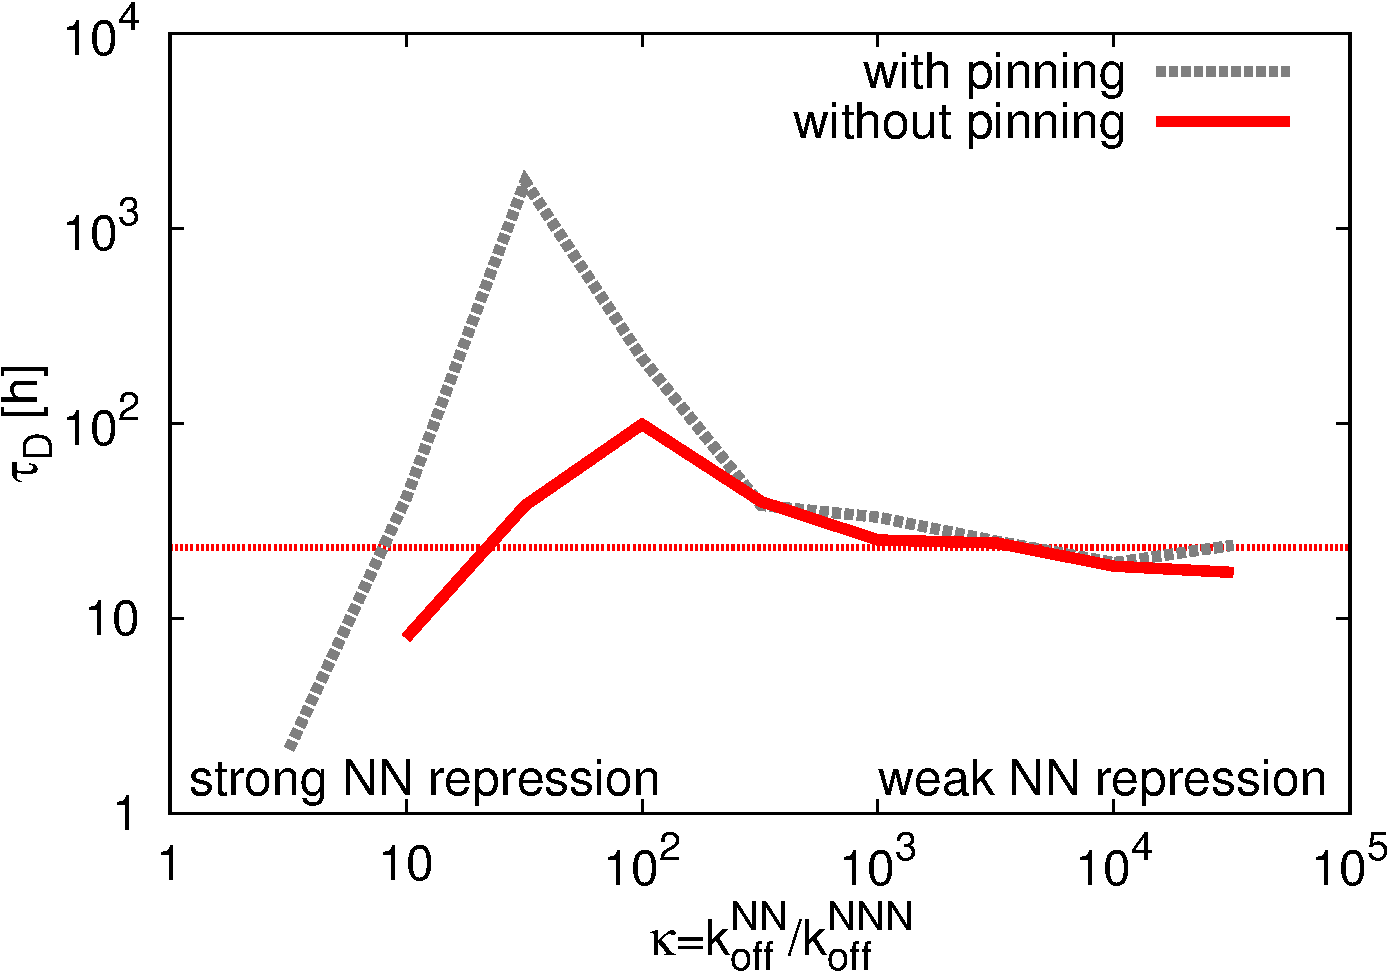
\includegraphics[width=0.66\textwidth]{Figures/FigureStabilityUnpinned.pdf}
%     \label{Fig-StabilityUnpinned}
%   }
    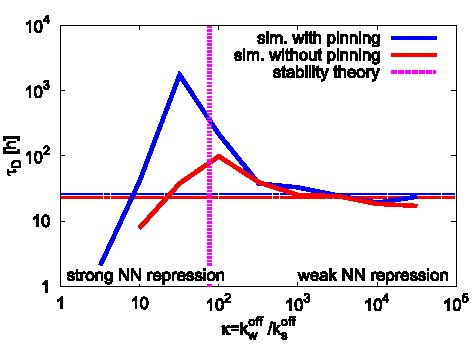
\includegraphics[width=0.8\textwidth]{Figures/FigureStabilityGrouped.pdf}
    \label{Fig-StabilityGrouped}
  \caption{
\textbf{An optimal strength of nearest neighbor repression maximizes pattern stability.}
	  %(\subref{Fig-StabilityGrouped})
	  The mean time until pattern destruction $\tau_D$ as a function of $\kappa$, 
	  the ratio between the weak and strong repressor off-rate, for the system in which expression 
	  of gene $\GA$ is fixed at the boundaries.
	  We observe a pronounced maximum of the stability time when the weak repression is about
	  30 times weaker than the strong repression ($\kappa_{\rm opt} = 31.6$) in the system with pinning at the boundaries (blue line).
   When pinning of the pattern at the system boundaries is relaxed (red line), the maximum of stability time moves to $\kappa = 100$.
   The dashed horizontal lines indicate the values for the completely uncoupled systems with $\kappa = \infty$.
   The dashed vertical line (magenta) shows the optimal repression strength ratio predicted analytically by our stability theory, $\kappa_{\rm theor} \simeq 76$ (see last part of Results section).
% 	  (\subref{Fig-StabilityUnpinned})
% 	  The same quantity for the system without pinning of $\GA$ at the system boundaries.
% 	  For comparison we replot the data for the system with pinning (gray dashed line).
% 	  In the system without pinning stability is maximized at an optimal NN repression strength ratio as well.
% 	  Note however that here the optimum slightly shifts towards weaker repression ($\kappa_{\rm opt}\simeq100$),
% 	  while the optimal pattern persistence time is significantly reduced as compared to the case with pinning.
% 	  Both curves agree well in the limit $\kappa\rightarrow\infty$.
	  %The system size is 8x40 nuclei, the typical copy number per nucleus $\simeq$ 15, kinetic parameters as described in Table \ref{Tab-Parameters}.
  \label{Fig-Stability}
}
\end{figure}

By quantifying pattern stability time, we found that $\tau_D$ depends strongly on the repression strength ratio, with a maximum of $\tau_D$ as a function of $\kappa$ at $\kappa_{opt}\simeq30$, see Fig. \ref{Fig-Stability} (blue curve). For $\kappa$ values close to $\kappa_{opt}$ pattern stability is still markedly enhanced.
While significantly less stable than in the region around the optimum, patterns with stability time on the order of several hours remain possible in the absence of NN repression ($\kappa\rightarrow\infty$). In contrast, when NN and NNN repression have close to equal strength ($\kappa\rightarrow 1$) patterns collapse almost immediately.

\mysubsubsection{In the maximally stable regime restoring forces reconstitute perturbed patterns}

The observation of a phase space region in which system trajectories persist for long times raises the question whether this region constitutes a true metastable basin of attraction.
%One way to determine whether there exists a basin that protects the pattern from destruction would be to compute the generalized free energy $F_g(\myvec\lambda)=-\log \rho_{SS}(\myvec\lambda)$ from the stationary distribution $\rho_{SS}(\myvec\lambda)$, as in \cite{Warren2005}. However, because the destroyed pattern effectively acts as a sink and the existence of a barrier which would allow for a quasi-stationary distribution within the basin of intact patterns cannot be assumed a priori, we cannot meaningfully compute such a stationary distribution.
We first addressed this question next by analyzing transient behavior of the perturbed patterns.
If enhanced phase space density in certain regions of the $(\lambda_{AC}, \lambda_{BD})$-space were indeed due to the presence of a metastable basin, perturbations that transiently drive the system away from the stable pattern should be counteracted by restoring forces.
%\noindent The observation of a phase space region in which system trajectories persist for long times indicates the presence of metastable basin of attraction. However, it remains unclear whether transient perturbations in gene expression that drive the system away from its stable pattern are counteracted by restoring forces in all directions of $(\lambda_{AC}, \lambda_{BD})$-space, or alternatively, there are direction in which perturbations are deteriorating the pattern without compensating forces.
To test this hypothesis, we perturbed relaxed five-stripe patterns from the hypothetical basin by artificially enlarging domains in which one gap gene is dominant. Using these perturbed states as initial conditions, we then ran the spatial-stochastic simulator with higher time resolution, and checked whether the perturbed systems relax back into the presumed basin.
We investigated two types of asymmetric perturbations: ``\GC expansion'', in which the central \GC domain is unidirectionally expanded at the expense of the posterior \GA domain, and the converse ``\GA expansion'', in which the anterior \GA domain is enlarged at the expense of the \GC domain. The perturbation experiments are described in detail in the Methods, Sec.~\ref{sec-GG-Methods}, and the Supporting Information.

We find that at $\kappa=\kappa_{opt}$, for both perturbations the perturbed pattern ensembles relax back to their original positions on a timescale $\sim 10~h$ (see Supporting Fig.~S1). This demonstrates that for optimal repression strength ratio an effective restoring force counteracts deviations from the five-stripe pattern for varied $\lambda_{AC}$.
Moreover, this suggests that the probability-enriched region within $R_S$ is a real metastable state confined by an underlying force field.
In accordance, the timescale of relaxation is orders of magnitude shorter than the timescale of pattern collapse.
Thus, for $\kappa=\kappa_{opt}$ pattern destruction is a Markovian transition between metastable basins with transition waiting times much longer than the timescales of intra-basin dynamics.
In contrast, we could not observe clear restoring behavior in the systems with very weak or no nearest neighbor interaction.
% (data not shown) \TODO{We should show this. Possibly SI or extend Fig. 5, we should avoid 'data not shown'}.
Here perturbations of similar strength tend to result in almost immediate pattern destruction.

In summary, for the repression strengths ratio $\kappa_{opt}\simeq30$ that maximizes stability, pattern breakdown appears to be an activated process characterized by a restoring force towards the initial state.

%%%%%%%%%%%%%%%%
%%% FIGURE 6 %%%
%%%%%%%%%%%%%%%%
\begin{figure}[h!]
  \centering
  \makebox[\textwidth][c]{
  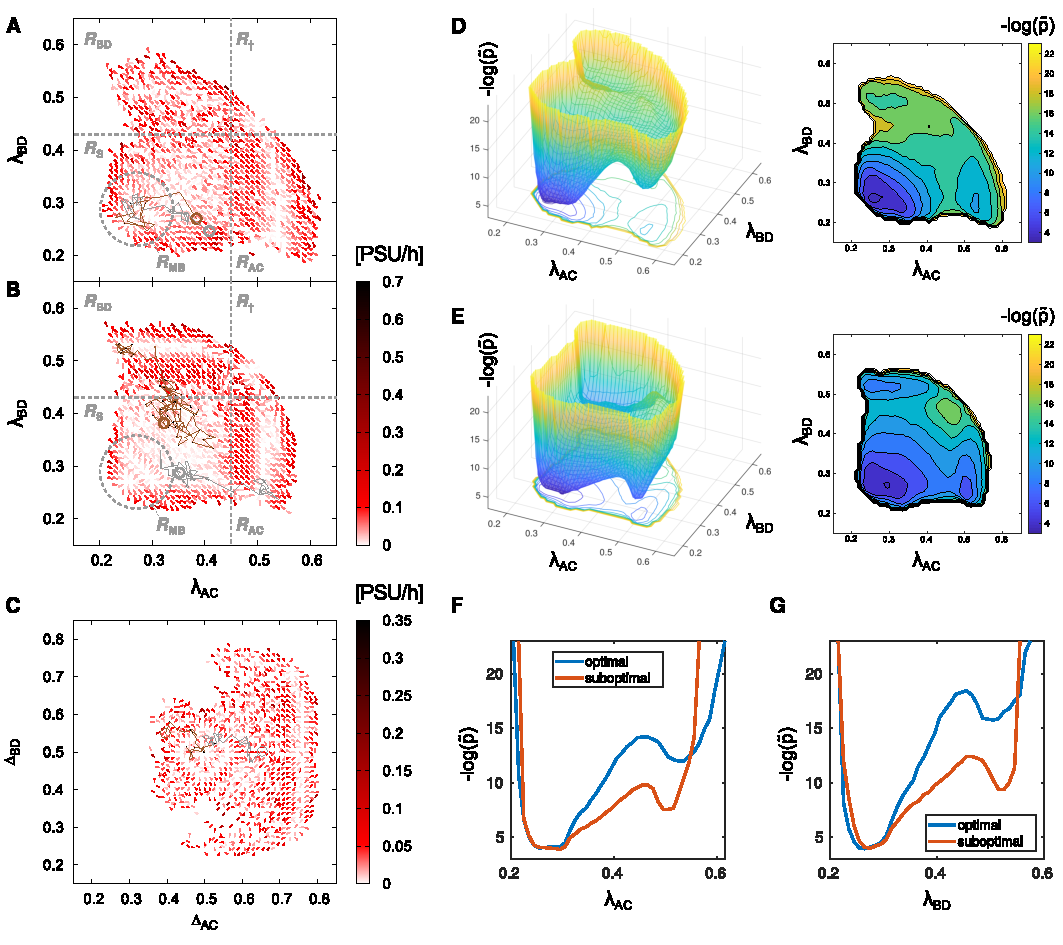
\includegraphics[width=1.0\textwidth]{Figures/FigureVelocities+BasinsV2.pdf}
  }
  \caption{
  \textbf{Phase space velocity fields and passage statistics reveal metastable basins.}
  \textbf{A}, \textbf{B})  Average phase space velocity fields for the system with optimal ($\kappa=\kappa_{opt}$, A) and suboptimal ($\kappa=1000$, B) repression strength ratio, in the phase space spanned by asymmetry factors $\lambda_{AC}$ and $\lambda_{BD}$ as defined in \eqref{eq:lambdaACBD}. The small subregion with concentrically inwards-pointing velocities towards which perturbed trajectories relax, corresponding to metastable basin of five-stripe patterns, is indicated ($R_{MB}$, dashed circle). Velocity fields were obtained by averaging displacements of all trajectories that exit the local bin (see Methods, Sec. \ref{sec-GG-Methods}). Two examples of trajectories relaxing after perturbations are shown (gray and brown lines) with their starting points (circles). The boundaries of phase space regions (thin dashed lines) are as in Fig.~\ref{Fig-DensityPinned}. Velocity magnitude is indicated with colors. \textbf{C}) The velocity field corresponding to $\kappa=\kappa_{opt}$ for the alternative asymmetry factors (``differences'') $\delta_{AC}$ and $\delta_{BD}$, as in \eqref{eq:deltaACBD}. 
  %A value of $x$ PSU/h indicates that on average trajectories passing through the respective phase space bin would increase the linear combination of the orthogonal asymmetry factors by $x$ if it could continue deterministically in a straight line for 1 hour of simulated time.
  In C the metastable basin $R_{MB}$ is localized around the center $(\delta_{AC},\delta_{BD})=(\frac{1}{2},\frac{1}{2})$, corresponding to a perfectly symmetric pattern. The magnitude unit ``phase space unit per hour'' (PSU/h) is specific to the chosen asymmetry factors.
  \textbf{D}, \textbf{E}) The landscapes of the ``pseudopotential'' $-\log \tilde{p}$ computed from the total number of phase space trajectories registered in the respective bin of the phase space.
  %The small plots to the right of the 3D views show sections through the landscapes along the $\lambda_{AC}$ and $\lambda_{BD}$ axes at the following values of the respective perpendicular coordinate $\lambda_{\perp}$ ($=\lambda_{BD}$ for $\lambda_{AC}$ and vice versa): 0.27 (blue), 0.28 (red) and 0.29 (yellow).
  The contour plots to the right of the 3D views show a projected view of the same landscapes.
  \textbf{F}, \textbf{G}) Comparison of sections in $\lambda_{AC}$ and $\lambda_{BD}$ directions, respectively, at $\lambda_{\perp}=0.28$ between the optimal and suboptimal choice of the repression strength ratio $\kappa$. Here the $-\log \tilde{p}$ profile is almost identical in the metastable basin $R_{MB}$, but transitions towards the destroyed pattern states face a higher barrier in the system with optimal $\kappa = \kappa_{opt}$, in both phase space directions.
  \vspace{1EM}
  \label{Fig-VelocitiesComparison}
  }
  %Panels A and B show that regions of enhanced phase space density (cf. Fig.~\ref{Fig-DensityPinned}) typically correspond to regions with low drift magnitude. %TO the main text?
  %up to a distance of $\sim 0.15$ phase space units from $P_0$;  trajectories attempting to leave this region are therefore, on average, quickly thrown back into the basin, towards $P_0$.   The basin cannot be identified any more in the system with suboptimal repression strength ratio (panels B and D); as especially visible in panel D, here the concentric pattern is replaced by a broad region of small average velocities with random orientation.

\end{figure}
%\FloatBarrier

%%%%%%%%%%%%%%%%
%%% FIGURE 6 %%%
%%%%%%%%%%%%%%%%
% \begin{figure}[ht!]
%   \centering
%     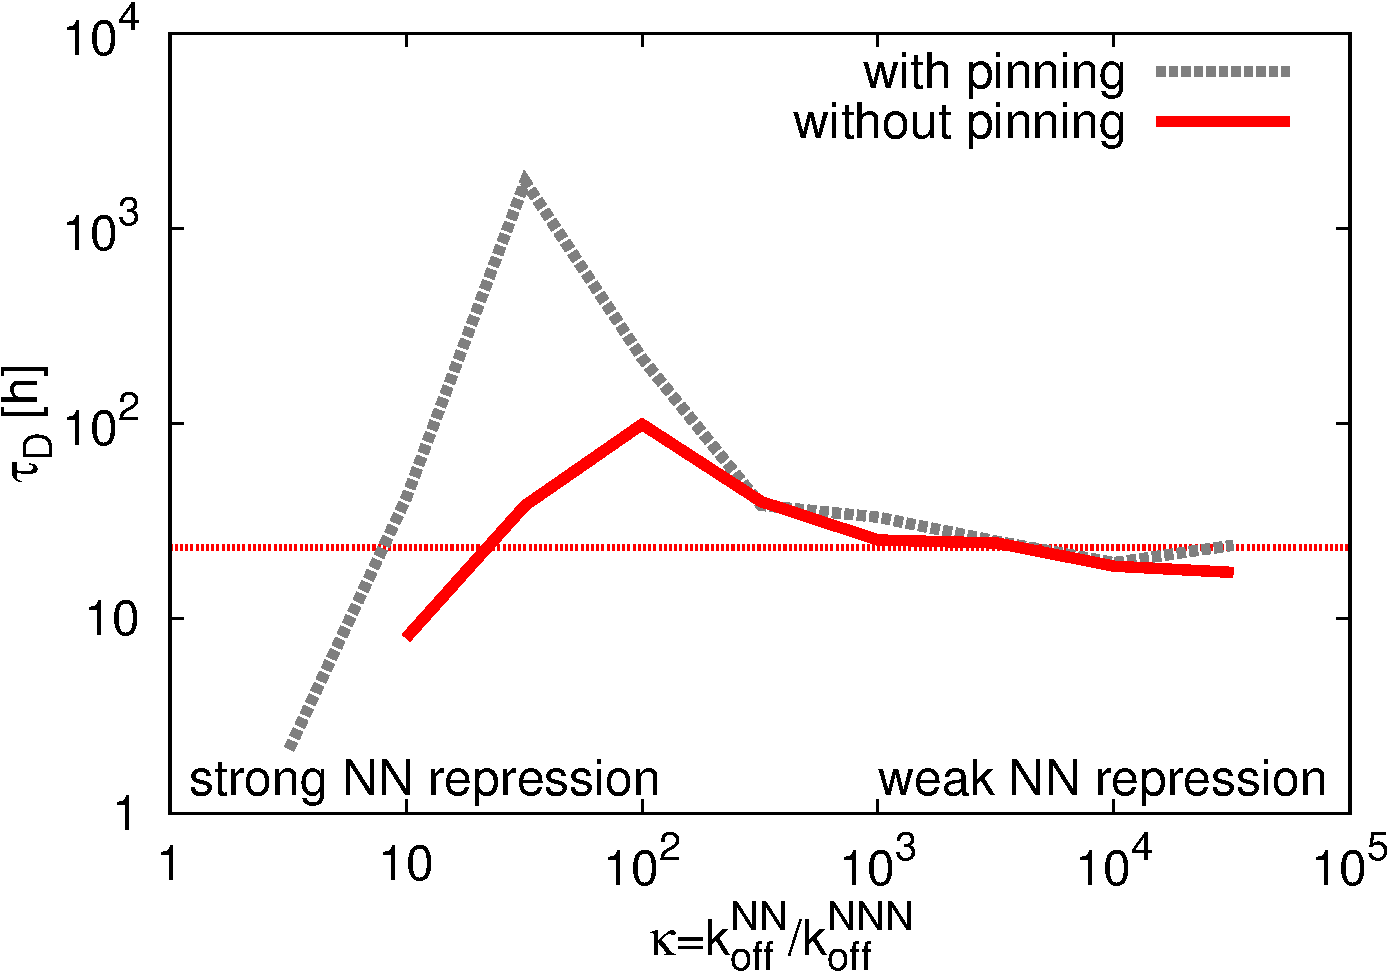
\includegraphics[width=0.75\textwidth]{Figures/FigureStabilityUnpinned.pdf}
%     \label{Fig-StabilityUnpinned}
%   \caption{
% \textbf{Maximization of pattern stability does not require pinning.}
%     Here we plot the mean time until pattern destruction $\tau_D$ as a function of $\kappa$, the ratio between the weak and strong repressor off-rate,
%  	  for the system {\it without} pinning of $\GA$ at the system boundaries.
%  	  For comparison we replot the data for the system with pinning (gray dashed line).
%  	  In the system without pinning stability is maximized at an optimal NN repression strength ratio as well.
%  	  Note however that here the optimum slightly shifts towards weaker repression ($\kappa_{\rm opt}\simeq100$),
%  	  while the optimal pattern persistence time is reduced compared to the case with pinning.
%  	  Both curves agree well in the limit $\kappa\rightarrow\infty$.
% 	  The system size is 8x40 nuclei, the typical copy number per nucleus $\simeq$ 15, kinetic parameters as described in Table %\ref{Tab-Parameters}.
%    \ref{Tab-GG-SI-Parameters}.
%   \label{Fig-StabilityUnpinned}
% }
% \end{figure}

\mysubsubsection{Statistical analysis of phase-space dynamics reveals a metastable basin}

\noindent We further figured that the existence of a true metastable basin should manifest itself also in the statistics of transient dynamics in phase space.
Here the local velocities in the $(\lambda_{AC}, \lambda_{BD})$ phase space are particularly informative:
forces that drive trajectories back into basins of attraction should translate into local mean phase space velocities with a clear bias towards the bottom of the basin.

To extract the velocity field for our system we modeled the coarse-grained pattern dynamics as overdamped  diffusive motion in the $\vecA \lambda \equiv (\lambda_{AC}, \lambda_{BD})$ plane, assuming that these degrees of freedom capture the slowest time scales of the system and making a Markov approximation for the fast dynamics \cite{Zwanzig1961, Mori1965}.  
This technique has been successfully applied in protein folding \cite{Yang2006, Kopelevich2005, Hummer2003, Plotkin1998}.
The corresponding model equation is
\begin{align}
 \frac{d}{dt} \vecA \lambda  = \avg{\vecA v_\lambda}(\vecA \lambda) + \sqrt{2D_\lambda(\vecA \lambda)} d\vecA W
\end{align}
where $\vecA W$ is uncorrelated (2D) white noise with unit covariance.
We estimated the local drift $\avg{\vecA v_\lambda}(\vecA \lambda)$ and diffusion coefficient $D_\lambda(\vecA \lambda)$ from our reweighed simulated trajectories by averaging local displacements (see Methods, Sec. \ref{sec-GG-Methods}, and Sec. S1.2 in the \SI).
%Note that the mean velocity $\avg{\vecA v_\lambda}(\vecA \lambda)$ is different from the gradient of the log of the stationary density  $\rho_{SS}(\vecA \lambda)$, which is not sampled in our simulations, and from the probability flux in stationary state.
Furthermore, $\avg{\vecA v_\lambda}(\vecA \lambda)$ is proportional to the effective force acting at the reduced phase space point $\vecA \lambda$ in the overdamped Langevin model.
The local mean velocity field $\vecA v_\lambda(\vecA \lambda)$ is determined by 
the conditional transition probabilities $\pi(\vecA \lambda, \vecA \lambda')$ 
between states $\vecA \lambda$ and $\vecA \lambda'$, and thus can be extracted from our transient simulation data. The resulting average velocity field in the reduced phase space of $(\lambda_{AC},\lambda_{BD})$ for the optimal repression strength ratio ($\kappa=31.6$) is in Fig. \ref{Fig-VelocitiesComparison}A, and for suboptimal ($\kappa=1000$) is shown in Fig. \ref{Fig-VelocitiesComparison}B.
%Panels A and B of Fig.~\ref{Fig-VelocitiesComparison} show a comparison of the average velocity field in the reduced phase space coordinate sets $(\lambda_{AC},\lambda_{BD})$ and $(\delta_{AC},\delta_{BD})$,
%for the optimal repression strength ratio ($\kappa=31.6$) in the system with pinning of \GA expression at the boundaries.
%We also plot the relaxation of example trajectories starting from perturbed intact pattern states for the two considered perturbations (grey and brown), 
%and indicate boundaries between different attractor regions (fine dashed lines), as in Fig.~\ref{Fig-DensityPinned}.
%Interestingly, the region $R^\dagger_{BD}$ in which either \GB or \GD are lost, has no clear boundaries for optimal $\kappa=31.6$, and only for much larger $\kappa=1000$ corresponding to weak NN repression the attraction basin in this region can be delimited similar to Fig.~\ref{Fig-DensityPinned}.

Interestingly, in Fig. \ref{Fig-VelocitiesComparison}A one can identify two regions of $(\lambda_{AC},\lambda_{BD})$-space with low average velocities: 
one within the region of stable states $R_S$, the other within the region $R^\dagger_{AC}$ of states in which the \GC expression domain is lost. The region $R^\dagger_{BD}$ in which either \GB or \GD are lost, has no clear boundaries for optimal $\kappa=31.6$, and only for much larger $\kappa=1000$ a low-velocity plateau is clearly seen in this region (Fig.~\ref{Fig-DensityPinned}B).
Notably, in the lower-left corner of the $R_S$ plateau we notice a small region in which average velocities are significantly higher and all pointing inwards. We refer to this region as $R_{MB}$, and identify it as the metastable basin of intact, relaxed five-stripe patterns. In accordance, the two shown exemplary perturbed trajectories relax into $R_{MB}$ after randomly exploring the $R_S$ plateau, and remain confined to the $R_{MB}$ for later times (Fig. \ref{Fig-VelocitiesComparison}A). However, if the system drifts far away from $R_{MB}$, in the direction of $R^\dagger_{AC}$, the trajectories are quickly absorbed into $R^\dagger_{AC}$ once they reach the edge of $R_S$ characterized by high velocity components towards $R^\dagger_{AC}$.

In order to further investigate the low-velocity attraction basins and the high-velocity ridges that separate these basins, we use a different representation of pattern asymmetry, defining the shifted difference coordinates 
\begin{align}
\delta_{AC} \equiv \frac{1}{2}([\GA]_{tot} - [\GC]_{tot})/N + \frac{1}{2} \,, \qquad
\delta_{BD} \equiv \frac{1}{2}([\GB]_{tot} - [\GD]_{tot})/N + \frac{1}{2} \,.
\label{eq:deltaACBD}
\end{align}
These coordinates measure the deviation from a perfectly symmetric pattern $P_0=(\delta_{AC},\delta_{BD})=(\frac{1}{2},\frac{1}{2})$ in a way that retains information about which of the antagonistic genes becomes dominant. The corresponding average velocities in $(\delta_{AC},\delta_{BD})$-space are shown in Fig.~\ref{Fig-VelocitiesComparison}C. The low-velocity basin, corresponding to $R_{MB}$, occupies the central part of $(\delta_{AC},\delta_{BD})$-space in Fig.~\ref{Fig-VelocitiesComparison}C.
Accordingly, perturbed trajectories relax towards the region enclosed by concentric velocity vectors pointing towards $P_0$. This is in line with the Waddington picture of canalization \cite{Waddington1942, Waddington1959}, in which developmental stages are seen as successive attractors of the underlying dynamics with the five-stripe pattern representing such an attractor.

%\clearpage
In Fig.~\ref{Fig-VelocitiesComparison}B  we show the average velocity field for the case with weaker NN repression ($\kappa=1000$). Here the velocity fields are even more plateau-like in the region corresponding to weakly asymmetric patterns, and the characteristic concentric velocity pattern indicative of the basin in the optimal case cannot be clearly discerned any more in this case. In accordance, trajectories starting from perturbed patterns do not relax back and progress towards patterns with at least one domain lost.
%Thus, canalization requires a minimum level of NN repression in this system.

In addition to the average velocity fields of the registered phase space trajectories, the signatures of the metastable basins are also visible in the local phase space density sampled over many trajectories that explored the phase space during the whole sampled time interval, $p(\vecA\lambda)$. A suitable quantity for visualizing the corresponding phase space ``landscape'' is the negative logarithm of $p(\vecA\lambda)$; note that in an equilibrated, stationary system this quantity would be proportional to the energy (landscape) defining the stationary probability distribution of the system. Since our system is genuinely non-stationary, this relationship does not hold. Nevertheless we can consider our most stable systems transiently equilibrated in the metastable basins or origin and akin to stationary systems \emph{until} they irreversibly cross the barrier towards one of the basins corresponding to destroyed patterns. Notably, while the depth of these basins grows with the amount of simulated time after the destruction event, the height difference between the metastable basin of intact patterns and the barrier separating it from the destroyed patterns basin is entirely determined by the recurring properties of the destruction process, and not expected to change provided that sufficiently many destruction events have been recorded.

In Fig.~\ref{Fig-VelocitiesComparison}D and E we plot the ``pseudopotential landscape'' defined as $-\log(\tilde p(\vecA \lambda))$ for optimal $\kappa=31.6$ (D) and suboptimal $\kappa=1000$ (E), where $\tilde p(\vecA \lambda)$ is a locally smoothened version of $p(\vecA\lambda)$ which equalizes out small local spikes in $p(\vecA\lambda)$ but preserves the overall structure of the resulting landscape (see Methods for details). The small plots right of the landscape visualizations show sections through the landscapes in direction of the asymmetry factors $\lambda_{AC}$ and $\lambda_{BD}$ at chosen constant values of the respective orthogonal factor (see Fig.~\ref{Fig-VelocitiesComparison} caption). In both cases we can clearly identify the metastable basin of undestroyed patterns and a barrier separating it from the basins of (half-) destroyed patterns. The basin corresponding to the states in which either the B or D domain is lost is less pronounced for the optimal choice of $\kappa$ due to its lower accessibility, and---more importantly---separated by a higher barrier.
This is best seen in a more detailed explicit comparison of the sections through the landscapes, shown in Fig.~\ref{Fig-VelocitiesComparison}F. The comparison clearly reveals that the barrier separating the metastable basin of intact patterns from the basin in which the C domain is lost is both higher and wider for the optimal choice of $\kappa$, overall leading to a markedly lower rate of pattern destruction.

Taken together, the analysis of both the velocity fields and the empirically sampled phase space density demonstrate that the long-time confinement of phase space trajectories close to the five-stripe pattern at optimal NN repression is due to the existence of a metastable basin which impedes progress towards losing one of the domains by restraining the system from leaving the metastable basin. With decreasing strength of NN repression the basin gradually disappears, thus enhancing the probability of pattern deterioration.

\mysubsubsection{Stability enhancement does not require pinning}

\noindent To assess whether pinning of the \GA-domains at the system boundaries is necessary for the observed stability enhancement at intermediate NN repression, we repeated our simulations and analysis for a system without pinning.
In contrast to the system with pinning, here the promoters of gene \GA in the nuclei at the system boundaries can be inhibited by the repressors of \GA.
We found that also in the system without pinning, pattern stability is markedly enhanced by the presence of weak interaction partners between two strongly repressing gene domains.
In Figure \ref{Fig-Stability} the red curve shows the mean destruction time $\tau_D$ against the ratio of the repressor off-rates $\kappa$ for the system without pinning.
%\ref{Fig-Stability}
We again find the highest pattern stability at an optimal repression strength ratio $\kappa^{\rm (np)}_{\rm opt}=100$ (red curve), which is close to the optimum in the system with pinning ($\kappa_{\rm opt}^{\rm (p)}\simeq 30$, blue curve),
albeit with about 10 times lower overall stability times;
yet, these stability times are still about an order of magnitude larger than without fine-tuning of NN interactions.

Overall this demonstrates that enhancement of pattern stability by at least one order of magnitude is possible both with and without pinning of expression at the system boundaries.
However, pinning alters the proportion of destruction pathways that the collapsing patterns pursue; we discuss this effect in more detail in Sec.~S1.3 of the \SI.

\mysubsubsection{The optimal pattern stability regime is predicted analytically by a mathematical model of expression domain competition}
\label{Sec-StabTheory}
\noindent

The problem of pattern stability has been recently addressed analytically in \cite{Majka2023}, where general and exact stability conditions for a contact zone between two interacting domain boundaries were derived. In this section, we show that these stability conditions can be successfully employed in the current multi-gene system, in order to make a coarse-grained prediction of stabilizing parameters set. %In result, we confirm the crucial role of weak interactions for the pattern stability and we elucidate the deterministic component of system dynamics.

The major finding reported in \cite{Majka2023} is that for sufficiently strong interactions between two genes, a contact zone of well-defined width is established between two domains of gene expression. However, in general, this pattern is dynamic, as one domain can still shrink and the other grow in coordinated manner, which preserves the width of the contact zone. This means that the contact zone can undergo a drift. It was found that the velocity of this motion asymptotically tends to a certain constant value, determined by the system parameters. This defines an attractor of the pattern dynamics, as the drift velocity and the width of contact zone are restored if concentrations of gene expression products are perturbed. A special case of this behaviour are (perfectly) stable patterns, for which the drift velocity is exactly zero. In these systems patterns can survive infinitely long. Conversely, increasing deviations of the system parameters from the stabilizing values translate into growing drift velocity, which eventually destroys the pattern. %However, it is argued in \cite{Majka2023} that the low-velocity plateau surrounding stable systems in parameter space is wide, so even systems with non-zero drift can effectively fulfil their biological role over a finite period of time. 
While the systems simulated in this work are highly stochastic, their dynamics also incorporate the deterministic component, which is expected to follow the principles outlined in \cite{Majka2023}. Thus, the survival time of the patterns is not only hampered by noise, but also by that deterministic component, unless stability conditions are met. We therefore assessed whether the numerically determined optimal $\kappa_{\rm opt}$ coincides with the theoretically predicted values of $\kappa_{\rm theor}$ that ensure pattern stability. 

To this end we mapped the microscopic model used in our stochastic simulations onto the effective reaction-diffusion model analysed in \cite{Majka2023} (see Methods). With the necessary readjaustments, the adapted effective model equation reads
\begin{equation}
\partial_t X_2(x,t)= D~\partial_{xx} X_2(x,t)-\gamma X_2(x,t)+H~\boldsymbol\theta\left(1-\sum_{Y\neq X} \epsilon_{XY} Y_2(x,t) \right) ~,\label{eq:effdyn}
\end{equation}
where $X,Y\in\{A,B,C,D\}$ denotes the particular proteins, $X_2(x,t), Y_2(x,t)$ is the concentration profile of their respective dimers, $D$ is the diffusion constant, $\gamma$ the degradation constant, $H$ a production constant, and $\epsilon_{XY}$ are gene-gene interaction strengths. $\boldsymbol\theta(\dots)$ denotes the Heaviside step function, corresponding to steep Hill kinetics.
Note that the derivations in \cite{Majka2023} only apply to systems with size $L\gg\lambda$, where $\lambda \equiv \sqrt{D/\gamma}$ is the characteristic length of gene interaction. For the systems studied here, $\lambda\approx 8.62~{\rm nm}$, which is markedly smaller than the system size $L\simeq 340~{\rm nm}$, warranting application of the theory.

While the original theory in \cite{Majka2023} describes only the contact zone between exactly two domain boundaries, we can adapt it to the four-gene system studied here. Fig. \ref{Fig-TypicalOutput} shows that in the alternating cushions system there are only two types of contact zones: (i) between two strongly interacting genes with the third, weakly interacting gene, expressed in the background or (ii) between two weakly interacting genes, with all other genes having close-to-zero expression level. Thus, we will consider stability of both contact zone types separately.

%\FloatBarrier
In the type-(i) contact zone, the dynamics of gene expression is described by the effective equations
\begin{equation}
\left\{
\begin{gathered}
\partial_t X_2(x,t)= D\partial_{xx} X_2(x,t)-\gamma X_2(x,t)+H \theta\left(1-K_w^{-1}\frac{H}{\gamma}-K_{s}^{-1} Y_2(x,t) \right) \\
\partial_t Y_2(x,t)= D\partial_{xx} Y_2(x,t)-\gamma Y_2(x,t)+H \theta\left(1-K_w^{-1}\frac{H}{\gamma} -K_{s}^{-1} X_2(x,t) \right)
\end{gathered}\right.
\end{equation}
where we approximate that the third ``background gene", has a constant expression level over the contact zone. The equilibrium value of this expression level is $H/\gamma$. $K_w$ and $K_s$ are the weak and strong repression constants, respectively and they satisfy (cf. Eq.~\ref{Eq-kappa} and Methods, Sec. \ref{sec-GG-Methods}):
\begin{equation}
\kappa=\frac{K_w}{K_s}=\frac{k_w^{\rm off}}{k_s^{\rm off}} ~.
\end{equation}
Type-(i) contact zones are established between genes A and C (with B or D in the background) as well as between B and D (with C in the background). In the type-(ii) contact zone, the equations take the form:
\begin{equation}
\left\{
\begin{gathered}
\partial_t X_2(x,t)= D\partial_{xx} X_2(x,t)-\gamma X_2(x,t)+H \theta\left(1-K_{w}^{-1} Y_2(x,t) \right) \\
\partial_t Y_2(x,t)= D\partial_{xx} Y_2(x,t)-\gamma Y_2(x,t)+H \theta\left(1 -K_{w}^{-1} X_2(x,t) \right)
\end{gathered}\right.
\end{equation}
This contact zone emerges between genes A and B, B and C, C and D as well as D and A. 

 The general stability conditions derived in \cite{Majka2023} define a relation between the system parameters that ensures zero drift of the contact zone. Applied to the system studied here these conditions read:
\begin{align}
(1-|R_X|)^{\lambda}=(1-|R_Y|)^{\lambda}~, && -1\le R_{X}\le 1~, && -1\le R_Y\le 1, &&\textrm{sgn}~R_X=\textrm{sgn}~R_Y~,\label{eq:stabcond}
\end{align}
where
\begin{align}
%\lambda=\sqrt{\frac{D}{\gamma}},&&
R_X=\frac{-2\gamma^2\tilde C_X  -\epsilon_{XX} \gamma H }{\epsilon_{XY} H}-1~, && R_Y=\frac{-2\gamma^2\tilde C_Y -\epsilon_{YY}\gamma H }{\epsilon_{YX} H}-1~,\label{eq:effparams}
\end{align}
Equations \eqref{eq:stabcond} can be applied separately to the type-(i) and type-(ii) contact zones in order to identify the range of stabilizing parameters in each case. Subsequently, we will investigate whether these ranges overlap, as the entire pattern is only stabilized when both types of contact zones are stable at the same time. We specify the constants in \eqref{eq:stabcond} for each contact zone type as follows:
\begin{align}
(i)&& \tilde C_{X}=\tilde C_Y=1-K_w^{-1}\frac{H}{\gamma}~, && \epsilon_{XY}=\epsilon_{YX}=-K_s^{-1}~, && \epsilon_{XX}=\epsilon_{YY}=0~, \label{eq:type(i)}\\
(ii)&& \tilde C_{X}=\tilde C_Y=1~, && \epsilon_{XY}=\epsilon_{YX}=-K_w^{-1}~, && \epsilon_{XX}=\epsilon_{YY}=0~.\label{eq:type(ii)}
\end{align}
Notice that as we choose $D$, $\gamma$ and $H$ to be the same for all dimers, $R_X=R_Y$ for each contact zone, and the first and the last of stability conditions \eqref{eq:stabcond} are automatically satisfied. The remaining condition is $-1\le R_{X}\le 1$, which requires closer examination. 

Employing parameters \eqref{eq:type(i)} for the type-(i) contact zone and parameters \eqref{eq:type(ii)} for the type-(ii) contact zone in $-1\le R_{X}\le 1$, we obtain two sets of inequalities: 
%We can now determine the values of $K_s$ and $K_w$ that ensure stability of the gene expression pattern. In general, the pattern is stable provided that both type-(i) and type-(ii) contact zones are stable at the same time. We therefore look for a unified stability condition satisfying the separate conditions for both types. The associated inequalities read:
\begin{equation}
\begin{aligned}
(i)&& -1\le \frac{-2(1-K_w^{-1}\frac{H}{\gamma})\gamma}{-K_s^{-1} H}-1\le 1~,\\
(ii)&& -1\le \frac{-2\gamma}{-K_w^{-1}H}-1\le 1~.
\end{aligned}
\end{equation}
Solving these inequalities results in:
\begin{equation}
\begin{aligned}
(i) && K_w\ge \frac{H}{\gamma}~,~ && K_s\le \frac{1}{(\frac{H}{\gamma})^{-1}-K_w^{-1}}~, \\
(ii) && K_w\le \frac{H}{\gamma}~.
\end{aligned}
\end{equation}
These conditions show that the addition of weak interactions is instrumental for increasing system stability. On the one hand, the type-(i) contact zone is stable provided that the weak interaction strength $K_w^{-1}$ does not exceed $\left(H/\gamma\right)^{-1}$; otherwise it would prevent the expression of strongly interacting genes in this region. On the other hand, for the type-(ii) interface it is necessary that $K_w^{-1}$ is greater than $ \left(H/\gamma\right)^{-1}$, as this minimal strength of repression is required to prevent co-expression of both weakly interacting genes in the same region. This shows that in order to simultaneously stabilize both types of contact zones, one must negotiate between these two largely opposite goals. This trade-off can be achieved only for the most marginal value in both parameter ranges, $K_w=H/\gamma$. This highlights why in the alternating cushions architecture the weak interactions have to be fine-tuned for pattern stability; in contrast, but in line with the numerical findings, the strong interactions characterized by $K_s$ can be arbitrarily large, $K_s\le+\infty$. The simulations in this work were performed for $K_s\simeq0.003~{\rm \mu m^{-3}}$ with $K_w$ varied to obtain different $\kappa$ values, see Methods, Sec. \ref{sec-GG-Methods}. Calculated from these microscopic parameters, $H/\gamma\simeq0.23~{\rm \mu m^{-3}}$. The resulting theoretical value of $\kappa$ ensuring stability is $\kappa_{\rm theor} \simeq 76$. This number is of the same order of magnitude as the optimal $\kappa$ in the simulated stochastic systems, showing better agreement with the no pinning case ($\kappa_{opt}^{\rm (np)}\simeq 100$) than with the case with pinning ($\kappa_{opt}^{\rm (p)}\simeq 30$), see Fig. \ref{Fig-Stability}. %\TODO{possibly briefly discuss also the horizontal lines corresponding to $\kappa\rightarrow\infty$ that are also in Fig. \ref{Tab-GG-SI-Parameters}, but were not referenced in the text (or I missed that)}%In both cases, theoretical result could be effectively used as a seed, which would significantly reduce the numerical search time for optimal value.


\clearpage
\section{Discussion}

In many developing organisms, morphogen gradients provide a long-range positioning system by activating downstream patterning genes in a concentration-dependent manner.
Prominent examples are the gap gene system in \Drosophila, whose main maternal regulators are the
morphogen gradients of \Bcd and \Cad spreading along the embryo axis \cite{Surkova2008, Jaeger2004, Driever1988a, Driever1988b, Frohnhofer1986, Struhl1989, Macdonald1986, Schulz1995, Mlodzik1987},
and the vertebrate neural tube with \emph{Shh} and \emph{BMP}/\emph{Wnt} secreted from the opposite sides of the neural tube \cite{Balaskas2012,Briscoe2015,Bier2015,Kuzmicz-Kowalska2020,Exelby2021,Minchington2023}.
%All these gradients are exponentially decaying and therefore the positional information that they encode becomes imprecise far from the gradient source. In spite of this, in Drosophila the gap gene stripes form robustly in the posterior half of the embryo, where \Bcd levels have been measured to be very low \cite{Gregor2007a, Gregor2007b}, and persist even after the \Bcd gradient starts to disappear in developmental cycle 14 \cite{Drocco2011}.
%\TODO{Further examples, e.g. from neural tube?}
%This suggests that in addition to external regulation by morphogen gradients, additional mechanisms are at work for establishing and maintaining the expression pattern in a (partly) self-organized fashion. %[I removed this paragraph as both in Drosophila and in spinal cord there are other gradients that provide additional positional information in regions with a specific gradient having very low values, and we discuss different mechanisms]
For the Drosophila embryo, multiple studies have shown that mutual interactions between gap genes play a crucial role in abdominal segmentation \cite{Sokolowski2012,Jaeger2004,Dubuis2013,Manu2009PlosBiol,Surkova2008,Sokolowski2015,Kozlov2012,Crombach2012, Manu2009PlosCompBiol}, 
leading to the formation of stable domains with slow effective dynamics \cite{Vakulenko2009}. 
However, it remains unclear how such a system could be robust given the stochastic nature of gene expression and regulation. 
Moreover, it is observed that maternal regulators such as the Bcd gradient disappear while the expression patterns invoked downstream persist \cite{Surdej1998,Spirov2009}.

Here we asked whether a system of mutually repressing developmental patterning genes arranged in successive expression domains can indeed be stable over developmentally relevant time intervals without upstream morphogen gradients while facing unavoidable fluctuations in the expressed gene products. Such copy number fluctuations can induce bistable switching at the domain boundaries, resulting in stochastic movement of the boundary which ultimately can lead to destruction of one of the gene expression domains.
%Here we asked whether a system of mutually repressing developmental patterning genes arranged in successive stripes can indeed be stable over the required developmental time interval, and robust against perturbations, in the absence of any morphogen gradient.
We quantified the mean stability time of a five-stripe expression pattern formed by four interacting genes
in a stochastic model conceptually inspired by the posterior \Drosophila embryo in cycle 14
as a function of the repression strength between neighboring stripes.
To be able to simulate the breakdown of very stable patterns we employedNon-Stationary Forward Flux Sampling (NS-FFS), an enhanced sampling scheme for simulating rare events in non-stationary systems with transient dynamics \cite{BeckerAllenTenWolde2012}.
We find that for an optimal value of the repression strength between adjacent expression domains 
the stability of the pattern is increased by about an order of magnitude. 
This stability optimum can be traced back to the fact that bistable switching at the boundary between domains of strongly mutually repressing genes is inhibited 
by an intervening cushion domain of a gene that weakly represses both strong partners. 
This stabilizing mechanism works best if the spacer gene represses its nearest neighbors (NN) with moderate strength: 
very weak NN repression has no effect while strong NN repression globally destabilizes overlapping domains.
At the optimal repression strength ($\kappa=\kappa_{\rm opt}$) the cushion thus slows down the random motion of the domain boundary and subsequent pattern destruction.

Stability is enhanced even more, by one more order of magnitude, if expression of the outermost gene is pinned at the system boundaries,
which effectively anchors the whole expression pattern.
Such a situation may emerge when the outermost gene remains under control of maternal cues, such as maternally deposited mRNA,
while the other gene stripes form only by zygotic interactions.
In that case we find that five-stripe patterns form a metastable attractor of the dynamics with a restoring force that counteracts perturbations, such as non-perfect initial conditions. 
In the optimal stability regime, 
our observations are consistent with the Waddington picture \cite{Waddington1942,Waddington1959} of development as canalization into successive metastable states, with the ordered initial gap gene pattern representing one of the metastable states in this succession.
Earlier work already demonstrated that developmental attractors may emerge as an intrinsic property of the gene expression pattern established through mutual interactions \cite{ Manu2009PlosBiol,Manu2009PlosCompBiol}.
Here, we demonstrate that also without morphogen gradients metastable basins can arise and protect expression patterns against stochastic fluctuations.

%Our numerical results are recovered by an analytical approximation that confirms the presence of a pattern stability region. In the absence of noise, the stable boundary between two gene expression domains can exhibit small drift described by low-velocity plateau \cite{Majka2023}. Here, the effects of noise affect domain boundaries in a similar way, as boundaries also drift, with an important difference that the average velocity of this drift is zero \TODO{write about restoring forces; other connections}

Further insight comes from the application of the stability theory derived in \cite{Majka2023} to the model of four genes interacting in the alternating cushions scheme. In agreement with the simulations, these analytical calculations reveal that the presence of weak interactions is necessary for stabilizing the system and establishing long-surviving patterns. More specifically, theoretical analysis shows that requirements for stability of type-(i) contact zones (i.e. two strongly interacting genes with the third weakly interacting in the background) and type-(ii) contact zones (i.e. two weakly interacting genes with other genes at very low expression level) are to certain degree incompatible, and the agreement can be achieved only for the most marginal value of $\kappa=\kappa_{\rm theor}$ in the respective stability range for each type. As a consequence, simultaneously ensuring perfect stability of both contact zone types requires the fine-tuning of weak repression strength, quantified by the corresponding dissociation constant $K_w$. 
%simultaneously ensuring perfect stability of type-(i) contact zone (i.e. two strongly interacting genes with the third weakly interacting in the background) and type-(ii) contact zone (i.e. two weakly interacting genes with other genes at very low expression level) requires fine-tuning of the strength of weak repression, quantified by the corresponding dissociation constant $K_w$. Intriguingly, the theoretical intervals of $K_w$ that ensure stability of both type-(i) and type-(ii) contact zones overlap only at a single value. 
This analytical prediction of one optimal value of $\kappa$ is in qualitative agreement with the numerical simulations, which show a very sharp rise in the survival time of expression pattern near one particular value of $\kappa = \kappa_{\rm opt}$, see Fig. \ref{Fig-Stability}. 

\pagebreak
Quantitatively, the numerical $\kappa_{opt}$ and theoretical $\kappa_{theor}$ agree particularly well in the no-pinning case (for pinning: $|\kappa_{\rm opt}^{\rm (p)}-\kappa_{\rm theor}|/\kappa_{\rm opt}^{\rm (p)}=139\%$, for no-pinning: $|\kappa_{\rm opt}^{\rm (np)}-\kappa_{\rm theor}|/\kappa_{\rm opt}^{\rm (np)}=24\%$). This is in line with the assumptions of \cite{Majka2023}, in which pinning was also neglected. Differences between $\kappa_{\rm theor}$ and $\kappa_{num}$ are expected due to the nature of approximations employed in the mapping of microscopic model on its effective representation \eqref{eq:effdyn}. It is plausible that this discrepancy could be resolved by constructing an even higher-level stability theory that takes into account the spatial variability of all four genes in each contact zone.

The simulations carried out in this work are both highly stochastic and microscopically detailed. Yet, the approximate agreement between $\kappa_{\rm opt}$ and $\kappa_{\rm theor}$ suggests that the deterministic dynamics of the generic model \eqref{eq:effdyn}, described in \cite{Majka2023}, is still important for this system. This deterministic theory suggests that, unless the system parameters are chosen to satisfy the stability conditions perfectly, the contact zones between the domains undergo drift, which would be able to eventually destroy the pattern on its own. This behaviour is overshadowed by strong stochastic fluctuations in the numerical simulations, but the significant increase in survival time in the vicinity of $\kappa_{\rm theor}$ suggests that nearly perfectly stable systems are significantly more robust against noise. However, the presence of noise seems to prevent perfect stability, as the increase of pattern survival time near $\kappa_{\rm theor}$, though remarkable, was finite in all simulations. Nevertheless, taken together, these results demonstrate that the stability theory might provide useful information also in the context of gene expression models with substantial levels of noise.

%However, as the velocity of this drift is slowest in the vicinity of the optimum, this regime results in long survival times. In accordance, in our simulations the survival time is markedly longer for $\kappa$ values lying in the vicinity of $\kappa_{theory}$. %Thus, the theoretical and numerical pictures are in qualitative agreement.
%\TODO{Maciek: check if this paragraph is well rewritten now.}

%Importantly the current simulations are highly stochastic, which is not directly included in the analytical framework of \cite{Majka2023}. The comparison of results indicates that noise might overshadow the asymptotically constant-velocity dynamics of domain pattern, claimed in \cite{Majka2023}. It also suggests that noise might prevent perfect stabilization even for optimal parameters, as in all simulations the observed survival time of pattern was finite. However, the existence of optimal $\kappa_{\rm opt}$, for which survival time increases sharply, suggests that the influence of noise is significantly attenuated near $\kappa_{opt}$. Taken together, it demonstrates that stability theory might provide useful information also in the context of gene expression models with substantial levels of noise. \TODO{I agree with PRtW that this paragraph needs to be rewritten as well.}


%These results indicate that $\kappa_{\rm theor}$ could be efficiently employed as a seed in the numerical search for the precise value of optimal $\kappa$. %%% I took this out because it may prompt reviewers to ask us about why we did not do it... ;-) [Tomek]
%This shows the potential of stability theory as a mean to facilitate the \textit{ab initio} pattern prediction.

The observed stability times appear sufficient for early fly embryogenesis  ($\simeq 2 h$ until cycle 14) for all NN repression strengths weaker than the optimal value, 
with or without pinning, even for the reduced system size considered here for computational feasibility.
%To assess the effect of system size, we have performed exemplary simulations in which we increased the gap gene production rate, the length of the system and its circumference, respectively (not shown) [ remove 'not shown', re-phrase or show this data].
%In all cases we find that while overall pattern stability is further increased, a stability maximum at intermediate NN repression strength persists. 
In a more realistic description, stability times will be likely modified due to the influence of system size. We expect that as expression domains grow in spatial extension or maximal copy numbers stability will be further enhanced. In the first case, stability is enhanced because more local cell fates need to be switched while the noise level remains the same. In the second case, the relative noise level is reduced in the first place.
%This expectation is supported by the following reasoning, larger domains persist for longer times compared with the default size domains when subject to the same level of noise in the gene expression.
Nevertheless, based on the theoretical and numerical evidence we believe that the stability enhancing mechanisms uncovered in this study will also apply to biologically relevant system sizes. Other factors potentially affecting stability are autoactivation interactions and interactions with other genes not included in the simplified regulatory network studied here, which will likely affect the dynamics of the gene expression pattern. Note, however, that the adapted stability theory clearly identifies the weak nearest-neighbor repression strength as the key parameter for enhancing stability, while the strong repressive interactions are found not to affect stability as long as they are chosen strong enough.

%and of features of gene regulation that were not included here (such as autoactivation and bursty translation);

In developmental perspective, the present work leads to the interesting question of how a properly ordered stripe pattern of mutually repressing genes is established initially. While pinning at the system boundaries can break the pattern symmetry between the genes forming the innermost and outermost stripes, additional symmetry breaking mechanisms would be required to position the remaining two genes. It is conceivable that the timing of the onset of gene expression for the different gap genes may determine their initial arrangement, which then gets stabilized by mutual interactions.
%Moreover, as the development of Drosophila embryo progresses the gap gene expression pattern is interpreted by downstream pair-rule genes, opening possibilities for studying the patterning precision that needs to be maintained in the upstream gap gene pattern to specify the downstream pair-rule pattern with positional precision observed in the experimental data \cite{Petkova2019}.  %%% I am not sure we want to keep the last sentence. Does it really add to our story? At least we need to reformulate. [Tomek]

The stabilizing mechanism arising from fine-tuning nearest-neighbor interactions in the alternating cushions scheme can be also considered in the broader class of regulatory mechanisms providing pattern stability against intrinsic and extrinsic noise \cite{Simsek2022,Iyer2022,Averbukh2017}. In future studies, it may be instrumental to further numerically and analytically explore the proposed model by including other biologically relevant features. Possible extensions include growth of the tissue by cell divisions, self-correcting mechanisms through cell-to-cell communication other than diffusive exchange of proteins, or inclusion of more specific noise types. These extensions could further test the validity of our stability under more realistic biological conditions. However, due to the remarkable agreement between our adapted stability theory and the numerical simulations of the minimal model studied in this work, we believe that more realistic variants of it will result in quantitative but not qualitative changes in our predictions.
%Taken together, the proposed stability mechanism can be relevant in computational models that quantify dynamics of spatiotemporal patterns emerging through gene-gene interactions in developing tissues.


\clearpage
\section{Methods}
\label{sec-GG-Methods}
\subsection*{Details of the model}
Our model is inspired by arguably the most paradigmatic developmental system
in which development of distinct cell fates is determined by local protein expression
patterns driven by external morphogen gradients, the early embryo of the fruit fly {\it Drosophila melanogaster}.
We model the egg-shaped embryo with its cortical layer of nuclei as
a cylindrical array of reaction volumes coupled by diffusion of proteins.
Every volume (nucleus) contains four individual promoters for each of the genes
\GA, \GB, \GC and \GD.
Each promoter can be repressed by the products of the three others with
different affinities; this system of four mutually inhibiting genes represents the gap gene system in the early fly embryo, formed by the four genes \hb, \kr, \kni and \gt, and comprises its essential regulatory interactions.
For combined repressive interactions, we employ OR-logic, i.e. whenever one of the three repressor sites is
occupied expression of the gene is completely blocked.
There is no competition for repressor sites on the promoters.
In the unrepressed state the promoters exhibit constitutive
protein production, i.e. no external activator signal is required.
This deliberately mimics a situation in which activation of the genes
is not provided by external morphogen gradients but by either an omnipresent
master activator or auto-activation with a low activation threshold.
Consequently, our model explicitly does not include morphogen gradients.
As a simplifying assumption, we treat the whole production process, 
i.e. transcription, elongation and translation, as one step governed by a single rate $\beta$.
Proteins however can form (homo)dimers and dedimerize again \cite{McCarty2003,Sauer1993},
and only in their dimeric form they act as repressors.
This is to ensure that antagonistic genes form bistable pairs for sufficiently strong
mutual repression.
Initially, all simulations are set up in a stripe pattern similar to the
experimentally observed order in the embryo posterior, i.e.
\GA-\GB-\GC-\GD-\GA \cite{Surkova2008, Jaeger2004, Clyde2003}.
This implies a fixed definition of ``gene neighborhood'' to which we refer throughout
this paper: 
by nearest neighbors (NN) we mean the pairs (\GA, \GB), (\GB, \GC), etc.,
while the pairs (\GA, \GC) and (\GB, \GD) are considered next-nearest neighbors (NNN).
A key ingredient of our model is that nearest-neighbor repression is
weaker than repression between next-nearest neighbor domains 
(see ``Parameter choice'' in Methods).
By default we pin the expression of \GA at the system boundaries,
i.e. in nuclei on the two outermost rings of the cylinder the \GA promoter
is irrepressible, and therefore constitutively produces \GA proteins.
This is motivated by the fact that in the real \Drosophila embryo the gene \Hb is under strict control by
the maternal morphogen \Bcd throughout the anterior half \cite{Driever1989}, 
while in the posterior a second enhancer exposes \Hb 
to positive regulation by the maternal terminal system \cite{Margolis1995, Casanova1990, Weigel1990}.
We compare this system to a system in which there is no pinning and all nuclei are identical.

\subsection*{Simulations}
To perform rare-event sampling of the spatially resolved system we integrate our
``Gap Gene Gillespie'' (GGG) simulator used in previous work \cite{Sokolowski2012, Erdmann2009} 
with the NS-FFS scheme \cite{BeckerAllenTenWolde2012}.
NS-FFS is used to monitor and process a progress coordinate written out by GGG at regular simulation interrupts,
at which GGG trajectories are cloned and restarted in a way that sampling is enhanced in the direction of increased 
progress coordinate, i.e. towards pattern destruction. \index{GGG} \index{Gap Gene Gillespie}

\subsubsection*{Spatially resolved stochastic simulations (GGG)}
In GGG, the model is implemented via the Stochastic Simulation Algorithm by Gillespie \cite{Gillespie1976, Gillespie1977}
on a cylindrical 2D lattice of reaction volumes at constant distance $l=8.5~\unit{\mum}$, with periodic boundary
conditions in the circumferential direction of the array. \index{Gillespie algorithm} \index{Stochastic Simulation Algorithm} \index{SSA}
%The different occupancy states of the promoters are treated as immobile chemical species with a maximal 
%copy number of one per nucleus and gap gene species.
An abstract graph of the reaction network that displays the set of reactions for any of the simulated promoters
is shown in Figure S8 in the \SI.
Diffusive chemical species (patterning gene proteins and their dimers) hop between neighboring volumes via the next-subvolume method 
\cite{Hattne2005} which integrates diffusion into the Gillespie algorithm by annihilation of a species copy in the volume of origin 
and instantaneous insertion of that copy in a randomly chosen neighboring volume with a rate $k_{diff}=4D_P/l^2$,
where $D_P$ corresponds to the protein diffusion coefficient.
The source code of GGG with examples can be downloaded from \myurl{https://github.com/YetAnotherTomek/GGG}.

\subsubsection*{Forward flux sampling}
We employ the recently developed non-stationary forward flux sampling (NS-FFS) method \cite{BeckerAllenTenWolde2012, BeckerTenWolde2012, Allen2005}
to enhance stochastic sampling of system realizations that increase a (reaction) progress coordinate $\lambda$ while retaining correct statistical weight.
NS-FFS achieves this by branching off multiple child trajectories upon crossing predefined interfaces in 
undersampled regions of $(\lambda,t)$-space and pruning trajectories that cross interfaces in oversampled regions.
%Pruning requires to recalculate the statistical weights of all trajectories of common ancestry with the pruned trajectory.
The NS-FFS scheme aims at equilizing the flux of simulated trajectories in the reaction coordinate direction among the time bins.
The rate of branching and pruning is calculated from the temporal trajectory crossing statistics collected during runtime.
To that purpose the time domain is subdivided into equidistant time intervals.
For a detailed account of the reweighting procedure we refer to \cite{BeckerAllenTenWolde2012}.
\index{forward flux fampling} \index{Non-Stationary Forward Flux Sampling} \index{NS-FFS}

\subsubsection*{Progress coordinates}
The choice of a suitable progress coordinate is a critical step of the FFS technique.
Here, we seek to enhance progress of the simulated patterns towards their destroyed state.
The destruction events are in particular characterized by the disappearance of one of the partners 
within each of the strongly repressing gene pairs.
Progress towards destruction thus is accompanied by increasing pair asymmetry,
which can be quantified for each pair separately by the following two asymmetry factors:
\begin{align}
 \lambda_{AC} &\equiv \max([\GA]_{tot},[\GC]_{tot}) / N \\
 \lambda_{BD} &\equiv \max([\GB]_{tot}, [\GD]_{tot}) / N
\end{align}
where $N = [\GA]_{tot} + [\GB]_{tot} + [\GC]_{tot} + [\GD]_{tot}$ is the number of all proteins in the system.
Based on this we define our progress coordinate, which increases whenever asymmetry among any of the pairs is augmented, via
\begin{align}
 \lambda &\equiv \lambda_{AC} + \lambda_{BD} = \left[ \max([\GA]_{tot},[\GB]_{tot}) + \max([\GB]_{tot},[\GD]_{tot}) \right] / N	\;.
\end{align}

Since NS-FFS features multi-dimensional reaction coordinates we compared our standard choice to a setup in which the two 
components $\lambda_{AC}$, $\lambda_{BD}$ of the reaction coordinate $\lambda$ are treated as two separate reaction coordinates 
with an own set of interfaces each.
While an orthogonal pair of reaction coordinates captures the principal reaction paths in our system more accurately,
the acquisition of crossing statistics is prolongated because of the increased number of bins in these simulations,
and we did not find any substantial advantage of this choice in terms of branching behavior.
We therefore preferred the standard definition.
\index{progress coordinate} \index{reaction coordinate}

\subsubsection*{Combination of simulation methods}
In order to wrap NS-FFS around the GGG simulator we run GGG for a predefined
simulation time $t_{GGG}=60~\unit{s}$. 
At the end of the simulation the reaction coordinates are calculated
and passed on to the NS-FFS module, and the end state of the simulation is recorded.
The NS-FFS module then determines whether an interface crossing has occured and, if so,
decides on whether the trajectory shall be branched or pruned.
In case of branching NS-FFS will prompt $n_B \geq 1$ restarts of the GGG simulator
with the recorded end state as initial condition, different random seeds and with new statistical weights.
At each crossing and at measuring times spaced by a regular interval $\Delta t$ the time, branch weight
and reaction coordinate values are stored in a tree-like data structure that facilitates later analysis.

Trajectory trees are started from a standartized, regular-stripe initial condition passed to the first call of GGG.
Propagation of the tree stops when all child branches have either reached the end of the time histogram or have been pruned.
Subsequently a new tree is started with a different random seed.
NS-FFS monitors the cumulative simulated time $T_{cum}$ and terminates simulation
when $T_{cum}$ exceeds a predefined maximal simulation time $T_{max}$ and the last 
trajectory tree has been propagated towards the end.
Typically, $T_{max}=3-7~\unit{h}$ and $T_{cum}=2-5\cdot10^{7}~s$,
which usually results in several thousand independent starts from the initial condition.
%Note that for a fixed $T_{cum}$ the number of independent starts is determined by the intensity of branching.

By default we start from an artificial pattern consisting of five non-overlapping stripes with rectangular profiles
occupying an equal part of the total system length $L/5$ each and equal number of monomers (no dimers) in each nucleus
close to the expected total copy numbers.
We find that these initial patterns quickly relax towards typical metastable patterns, i.e. into the metastable main basin of attraction,
which justifies our approach a posteriori.


\subsection*{Parameter choice}

\subsubsection*{Repression}
We are mainly concerned about the importance of distinct repression strength of nearest-neighbor (NN)
as compared to next-nearest neighbor (NNN) interaction.
We assume repressor binding-rates to be diffusion-limited via $\kRon=4\pi\sigma_R D_N$,
where $D_N$ is the \emph{intranuclear} diffusion constant and $\sigma_R$ an effective target radius.
Repression strength therefore is varied by changing the unbinding rates of the repressing dimers.
The main parameter in our simulations is $\kappa=\kRoffW/\kRoffS$, the ratio between NN and NNN repressor off-rate.
In this work only $\kRoffW$ is varied, while $\kRoffS$ is chosen sufficiently low to guarantee bistability between next-nearest neighbor genes,
which is a precondition for the formation of individual stripe domains in the first place, see Table S1 in the \SI.
For $\kappa=1$ NN and NNN repressive interactions are equally strong,
while for large $\kappa$ values NN repression is much weaker than NNN repression.
In the ``uncoupled limit'' $\kappa\rightarrow\infty$ the two bistable pairs coexist without sensing each other.
We do not consider cases with $\kappa<1$.

\subsubsection*{Dimerization}
We set the dimerization forward rate $\kDon$ to be equal to two times the diffusion-limited repressor binding rate,
which is accounting for the fact that both reaction partners are diffusing.
The dimerization backward rate is set via $\kDoff=\kDon/V_N$ ($V_N$ = nuclear volume) as in \cite{Warren2004,Warren2005,Morelli2008,Sokolowski2012}
to ensure that at any moment most of the proteins are dimerized.

\subsubsection*{Production and degradation}
In our model both monomers and dimers are degraded.
This leads to a nontrivial dependence of the total copy number on production, degradation and (de)dimerization rates,
as we discuss with more detail in \cite{Sokolowski2012}.
Since we did not find any experimental reports of gap protein lifetimes, we chose equal monomeric ($\mu_M$) and equal dimeric degradation rate ($\mu_D$) 
for all genes and set these quantities to values that lead to a reasonable effective lifetime of the corresponding proteins of $t_{eff} \simeq 100~\unit{s}$.
The steady-state copy number is tuned via the production rate $\beta$.
By default, we consider copy numbers as low as possible ($\simeq 15$) to minimize computational effort.
The effect of increasing the average copy number is discussed in the ``Discussion'' section.

\subsubsection*{Geometry and internuclear transport}
The choice of our geometric parameters, in particular of the lattice constant, is inspired by experimental measurements
in the \Drosophila embryo by Gregor et al. \cite{Gregor2007a}.
Information on the diffusion constants of proteins involved in early \Drosophila patterning is scarce.
The diffusion constant of the morphogen \Bcd has been measured by several groups, 
yet its true value is still under debate \cite{Gregor2007b, Abu-Arish2010}.
In our model we therefore set for all patterning proteins an effective internuclear diffusion constant $D_P=1~\unit{\mumsps}$,
which comprises both protein import/export and actual diffusion.
This value is a reasonable cytoplasmic diffusion coefficient and well within the bounds reported for \Bcd.

The simulated lattice is 40 nuclei long so that the total system length $L$ roughly corresponds
to the posterior 2/3 of the \Drosophila embryo in cycle 14.
To reduce computation effort we simulate a system with smaller circumference (8 nuclei) as compared to the living embryo.
This is justified by the fact that for our standard diffusion constant $D_P$ and effective protein lifetime $\mu_{eff}$ 
the diffusive correlation length $l_{corr}=\sqrt{D_P/\mu_{eff}}$ is $\leq 2$ nuclei.
A larger circumference therefore is not expected to introduce new features into the system,
but might alter the timescales of expression boundary movement and domain desintegration.
We discuss the effect of reduced system size on measured stability times in the ``Discussion'' section.

A complete overview of the specific numerical values of our model parameters is found in Table~S1 of the \SI.


\subsection*{Data analysis}
\subsubsection*{Quantification of pattern stability}
%In order to analyse the pattern dynamics we produce two different 2D-histograms of the simulated trajectories: one histogram over the space spanned by the progress coordinate $\lambda$ and the simulation time $t$ and one over the reduced phase space spanned by the two components of the progress coordinate $\lambda_{AC}$ and $\lambda_{BD}$. Trajectories are binned with the statistical weight assigned by NS-FFS, and in the end the histograms are normalized.

In order to analyse pattern stability we represent each simulated pattern as a point in ($\lambda_{AC}$, $\lambda_{BD}$) phase space. For every pattern simulation from time $t=0$ until time $t=t_{\rm end}$ the temporal sequence of these points corresponds to a trajectory in the ($\lambda_{AC}$, $\lambda_{BD}$) space. For each parameter choice and pinning scenario, we restarted the simulations with 6000 trajectories started from the relaxed initial patterns at $t=0$; the trajectories ensemble is then further enriched by the branching process at the NS-FFS interfaces. Next, the trajectories are binned with the statistical weight assigned by NS-FFS, and then the histograms are normalized. As a result, we can identify a few distinct regions that accumulate probability. In order to formally define these regions we define rectangular boundaries that enclose accumulated probability regions corresponding to different types of patterns:
\begin{itemize}
 \item the metastable main basin with five-stripe pattern:\\
       $R_S\equiv\{(\lambda_{AC}, \lambda_{BD}) | {\lambda_{AC}\leq 0.45 \wedge \lambda_{BD}\leq 0.43} \}$
 \item the basin in which either the \GA or \GC protein domain was lost:\\
       $R^\dagger_{AC}\equiv\{(\lambda_{AC}, \lambda_{BD}) | {\lambda_{AC} > 0.45 \wedge \lambda_{BD}\leq 0.43} \}$
 \item the basin in which either the \GB or \GD protein domain was lost:\\
       $R^\dagger_{BD}\equiv\{(\lambda_{AC}, \lambda_{BD}) | {\lambda_{AC} \leq 0.45 \wedge \lambda_{BD} > 0.43} \}$
 \item the basin in which either \GA or \GC and one of \GB or \GD were lost:\\
       $R^\ddagger\equiv\{(\lambda_{AC}, \lambda_{BD}) | {\lambda_{AC} > 0.45 \wedge \lambda_{BD} > 0.43} \}$
\end{itemize}
%%% Version with equation numbers:
% \begin{itemize}
%  \item the metastable main basin of intact / undestroyed patterns:
%       \begin{align}
%        R_S\equiv\{(\lambda_{AC}, \lambda_{BD}) | {\lambda_{AC}\leq 0.45 \wedge \lambda_{BD}\leq 0.43} \}
%       \end{align}
%  \item the basin in which either the \Hb or \Kni domain has vanished:
%       \begin{align}
%        R^\dagger_{AC}\equiv\{(\lambda_{AC}, \lambda_{BD}) | {\lambda_{AC} > 0.45 \wedge \lambda_{BD}\leq 0.43} \}
%       \end{align}
%  \item the basin in which either the \Kr or \Gt domain has vanished:
%       \begin{align}
%        R^\dagger_{BD}\equiv\{(\lambda_{AC}, \lambda_{BD}) | {\lambda_{AC} \leq 0.45 \wedge \lambda_{BD} > 0.43} \}
%       \end{align}
%  \item the destroyed end states basin in which either \Hb or \Kni and one of \Kr or \Gt have vanished:
%       \begin{align}
%        R^\ddagger\equiv\{(\lambda_{AC}, \lambda_{BD}) | {\lambda_{AC} > 0.45 \wedge \lambda_{BD} > 0.43} \}
%       \end{align}
% \end{itemize}

Note that the location of the regions slightly changes for different values of $\kappa$.
We found that the above boundary definitions constitute a good compromise.
For each basin we compute the fraction of total probability as a function of time by integrating the weights of
trajectories that are within the basin at time $t$.
We define the \emph{pattern survival probability} to be the integrated probability in $R_S$ at time $t$ after initialization:
$S(t)=\iint_{R_S} p(t) d\lambda_{AC} d\lambda_{BD}$.
As expected, $S(t)$ displays roughly exponential decay behavior after a certain lag phase that can be attributed to initial relaxation.
To obtain the \emph{pattern destruction rate} $k_D$ we fit a function $f(x)\equiv \exp(-k_D(t-t_{lag}))$ to $S(t)$.
This only yields satisfactory results if the fitting range is adapted accordingly, i.e. only $S(t)$ values for $t>t_{lag}$ are taken into account.
Since $t_{lag}$ itself is a fitting parameter we adopted the following protocol:
Starting from a value of $t_{start}$ that is clearly in the relaxation regime we perform the fit on the interval $[t_{start}, t_{end}]$
where $t_{end}$ is the largest time recorded.
We then choose the fitted values $k_D$ and $t_{lag}$ for which $|t_{lag}-t_{start}|$ is minimal.
From this we compute the pattern stability time (average time until pattern has lost one of the domains) via $\tau_D \equiv 1/k_D$.
In most considered cases the patterns are very stable, i.e. $k_D$ very small, and we can expand
$S(t)\simeq 1 - k_D(t-t_{lag})$.
As a control, we therefore also fitted $g(t)\equiv k_D(t-t_{lag})$ to $1-S(t)$ for a fixed $t_{lag}$ clearly in the
exponential regime and obtained almost identical results.

\subsubsection*{Computation of average probability fluxes}
To quantify which destruction pathways are dominant we computed the average fluxes $J_{avg}$ into the regions of (partly) destroyed patterns.
Here the average flux is defined as the average rate of increase in time of the fractional probability in the region and
obtained by fitting a linear function $h(t)\equiv J_{avg} t + P_0$ to $P_R(t) \equiv \iint_R p(t) d\lambda_{AC} d\lambda_{BD}$
for $R \in \{R^\dagger_{AC}, R^\dagger_{BD}, R^\ddagger \}$ over the interval $[t_{start},t_{end}]$ with $t_{start}$ chosen such that $\partial_t P_R(t)\neq0$ for $t>t_{start}$.
$P_0$ depends on the particular choice of $t_{start}$ and is discarded.

\subsubsection*{Computation of average flux velocities}
The average local drift velocity and diffusion constant of the trajectories in the $(\lambda_{AC},\lambda_{BD})$ phase space
are computed by averaging displacements $\Delta \lambda_{AC(BD)}\equiv\lambda_{AC(BD)}(t+\Delta t)-\lambda_{AC(BD)}(t)$
and squared displacements $\Delta \lambda^2 \equiv \Delta \lambda_{AC}^2 + \Delta \lambda_{BD}^2$ on a two-dimensional lattice of bins
covering the whole phase space.
Displacements $\Delta \lambda_{AC(BD)}$ are assigned to the bin at $\vecA{\lambda} \equiv (\lambda_{AC}, \lambda_{BD})$,
i.e. we are averaging outgoing displacements and the averaged vector $\langle\vecA{\Delta\lambda}\rangle (\vecA{\lambda})$ 
therefore will represent the average velocity with which trajectories \emph{leave} this bin.
The local phase space diffusion constant is calculated as
$D_\lambda (\vecA{\lambda}) \equiv \frac{1}{4\Delta t} \left[ \langle\Delta \lambda^2\rangle (\vecA{\lambda})
  - \left( \langle\Delta\lambda_{AC}\rangle^2 (\vecA{\lambda}) + \langle\Delta\lambda_{AC}\rangle^2 (\vecA{\lambda}) \right) \right]$.
This is done in the same way for other combinations of phase space coordinates.
The diffusion-drift decomposition is explained in more detail in the \SI.

\subsubsection*{Computation of ``pseudopotential'' landscapes}
The trajectory binning procedure used for computing the average flux velocities as described above was at the same time used for computing the ``pseudopotential'' $-\log(\tilde p(\vecA \lambda)$. Herein $\tilde p(\vecA \lambda)$ is the local density calculated from the reweighed number of trajectories \emph{leaving} the bin at $\vecA \lambda = (\lambda_{AC},\lambda_{BD})$, and smoothened afterwards by 2D median filtering over $n_{filt}$ neighboring bins. For the 2D median filtering we used the \texttt{medfilt2} function from the MATLAB Image Processing Toolbox. We empirically chose $n_{filt}=4$ as we found that this choice efficiently removes local spikes in $p(\vecA \lambda)$ without changing the overall shape of the landscape.

\subsection*{Perturbation experiments}
Simulations starting from perturbed initial conditions were performed directly via the GGG simulator.
First the systems were relaxed to representative states within the metastable basin for a simulated time
of $t_{relax}=30~\unit{min}$.
%($60~\unit{min}$ for higher copy numbers). 
The final states of these runs then were post-modified according to the following two protocols:
\begin{enumerate}
 \item ``\GC expansion'': starting from mid-embryo the central \GC protein domain was expanded as follows:
	the configurations in the nuclei just posterior to mid-embryo were
	copied and used to overwrite configurations in the subsequent $\Delta$ rows in the axial 
	($z$-) direction of the cylinder. The original configurations were stored and for each nucleus at
	row $z_i > N_z/2+\Delta$ (counting from the anterior) the configuration was overwritten by 
	the original configuration at $z_i-\Delta$. The posterior-most nucleus was exempted from overwriting to preserve pinning.
 \item ``\GA expansion'': here the anterior \GA protein domain was enlarged at the expense of the \GC protein domain.
	To this purpose we applied the same copy-paste procedure as above starting form $z_i=5$,
	however only nuclei up to mid-embryo ($z_i \leq N_z/2$) were overwritten by the original configurations at $z_i-\Delta$.
\end{enumerate}
$\Delta$ quantifies the severity of perturbation. We found that $\Delta<4$ results in
changes to the pattern that were hard to distinguish from noise,
while for $\Delta > 12$ perturbations were large enough to induce immediate pattern destruction with high probability.
We therefore limited systematic tests to pertubations with $\Delta\in\lbrace 4, 8, 12 \rbrace$.
Starting from the perturbed initial conditions simulations were continued for $t_{sim}=20~h$ and
snapshots of the current configurations in all nuclei were written out with an acquisition interval 
of $10~\unit{min}$ (simulated time).
10 samples starting from 10 different perturbed initial conditions were produced for each set of parameters.

In order to overcome the difficulties of boundary detection we quantified the motion of protein domains
by tracking their center of mass (CoM) along the $z$-axis of the cylinder.
For each considered gene $G$ we define the CoM $z_G$ as
\begin{align}
 z_G &\equiv \frac{\int_z \int_r z G_{tot}(r,z) dr dz }{\int_z \int_r G_{tot}(r,z) dr dz}
\end{align}
where $G_{tot}=[G]+2[G_2]$ is the total copy number.
Since our system features two \GA domains we calculate $z_\GA$ separately for the anterior ($\GA_{ant}$)
and the posterior ($\GA_{post}$) part of the embryo by restricting $z$-integration adequately.
While the CoM remains unchanged upon symmetric changes of the domain boundaries or global copy number increase,
it is well-suited to indicate relaxations from the asymmetric perturbations that we apply.
To find general trends in the time-evolution of the domains CoM trajectories were averaged over the 10 samples.

\subsection*{Effective reaction-diffusion dynamics of dimer expression}

In this section we map the fully microscopic model defined in Fig.~\ref{Fig-ModelSketch} onto the effective model from \cite{Majka2023}. First, we postulate that the stochastic dynamics of gene expression studied in this paper corresponds to the following effective dynamical equations:
\begin{equation}
\begin{gathered}
\partial_t X_1(x,t)=-\mu_M X_1(x,t)-k_{on}^DX_1^2(x,t)+k_{off}^DX_2(x,t)+\beta f(\{Y_2(x,t)\}_{Y\neq X})~,\\
\partial_t X_2(x,t)=D_0\partial_{xx}X_2(x,t)-(k_{off}^D+\mu_D)X_2(x,t)+k_{on}^DX_1^2(x,t)~,
\end{gathered}\label{eq:start}
\end{equation}
where $X,Y\in\{A,B,C,D\}$ denotes the expressed protein species, $X_1$, $Y_1$ are the concentrations of its monomer, and $X_2$, $Y_2$ are concentrations of its dimers. The synthesis and decay of dimers is described by rates $k_{on}$ and $k_{off}$. Both, monomers and dimers degrade with rates $\mu_D$ and $\mu_M$. In this system, only dimers are allowed to diffuse (with diffusivity $D_0$) and only monomers are primarily synthesized, with maximal production rate $\beta$ and production kinetics described by function $f(\{Y_2(x,t)\}_{Y\neq X})$, which we specify later. However, we assume that in the absence of other dimers $Y_2\neq X_2$ the production is active by default, so $f(\{0\})=1$. Since the system has cylindrical symmetry, we will treat the axis $x$ as distinguished and treat the system as effectively one-dimensional.

The fact that the model defined by eqs. \eqref{eq:start} involves monomers and dimers complicates its mapping onto the model in \cite{Majka2023}. We therefore translate it into a simplified model, tracking the effective dynamics of dimers only. To this end, we will first determine the ratio between stationary concentrations $\tilde X_1$ and $\tilde X_2$ in the absence of other dimers ($Y_2(x,t)=0$) and assuming system homogeneity. In this case, equations \eqref{eq:start} turn into:
\begin{equation}
\begin{gathered}
0=-\mu_M \tilde X_1-k_{on}^D \tilde X_1^2+k_{off}^D \tilde X_2+\beta ~,\\
0=-(k_{off}^D+\mu_D)\tilde X_2+k_{on}^D \tilde X_1^2 ~.
\end{gathered}
\end{equation}
Solving for $\tilde X_1$ and $\tilde X_2$, we obtain:
\begin{equation}
\begin{gathered}
\tilde X_1=\frac{1}{2k_{on}^D}\left(-\frac{k_{off}^D+\mu_D}{\mu_D}+\sqrt{\frac{(k_{off}^D+\mu_D)^2}{\mu_D^2}\mu_M^2+4k_{on}^D \beta \frac{k_{off}^D+\mu_D}{\mu_D}} \right) ~,\\
\tilde X_2=\frac{\beta}{\mu_D}-\frac{\mu_M}{\mu_D}\tilde X_1 ~.
\end{gathered}
\end{equation}
We will now sum both equations in \eqref{eq:start} to obtain
\begin{equation}
\partial_t(X_1(x,t)+X_2(x,t))=D\partial_{xx}X_2(x,t)-\mu_D X_2(x,t)-\mu_M X_1(x,t)+\beta f(\{Y_2\}_{Y\neq X}) ~,
\end{equation}
and approximate
\begin{equation}
X_1(x,t)\approx \frac{\tilde X_1}{\tilde X_2} X_2(x,t) ~.
\end{equation}
In other words, we assume that $X_1(x,t)$ follows strictly $X_2(x,t)$. The advantage of this approximation is that it becomes exact in the stationary state. This procedure results in the following effective equation for $X_2(x,t)$:
\begin{equation}
\partial_t X_2(x,t)= D_X\partial_{xx} X_2(x,t)-\gamma_X X_2(x,t)+H_X f(\{Y_2\}_{Y\neq X}) ~, \label{eq:effectiveform}
\end{equation}
where the rescaled constants are:
\begin{align}
D_X=\frac{D_0}{1+\frac{\tilde X_1}{\tilde X_2}} ~, &&\gamma_X=\frac{\mu_D+\mu_M\frac{\tilde X_1}{\tilde X_2}}{1+\frac{\tilde X_1}{\tilde X_2}} ~, &&H_X=\frac{\beta}{1+\frac{\tilde X_1}{\tilde X_2}} ~.
\end{align}

We can now specify the kinetics function. The microscopic dynamics is such that each gene $X$ is produced, unless it is blocked by the biding of any other dimer to its repressor site on the promoter. In the averaged-out description, we expect that a sufficiently high concentration of free repressor particles effectively shuts down the production of $X$. Similarily to \cite{Majka2023}, we will assume that this transition is steep, so we can choose the functional form of the regulatory Hill function in \eqref{eq:effectiveform} to have the overall shape of Heaviside step function:
\begin{equation}
f(\{Y_2\}_{Y\neq X})=\boldsymbol\theta\left(\sum_{Y\neq X}\epsilon_{XY} Y_2(x,t)-C_X\right) ~. \label{eq:theta}
\end{equation}

Finally, we relate the effective gene interaction constants $\epsilon_{XY}$ to microscopic parameters by the following reasoning: In the microscopic simulations, the attachment of $Y_2$ to the repressor site is described by the constant $k_{on}^R$ and detachment by $k^{\rm off}_{\rm s}$ or $k^{\rm off}_{\rm w}$. Assuming that the repressor production speed can be approximated by Michealis-Menten kinetics, with the repressor site acting like a ``catalyst'', we know that
\begin{equation}
K_{Y}=k^{\rm off}_{\rm w,s}/k_{\rm on}^R
\end{equation}
where $k^{\rm off}_{\rm w,s}$ stands for either $k^{\rm off}_{\rm w}$ or $k^{\rm off}_{\rm s}$, is the concentration of repressor dimers $Y_2$ at which the velocity of production of $Y_1$ is at the half of its maximal value. We postulate that at this point $Y_2$ effectively switches off the production of $X$, and we equate this point with reaching the threshold for production in \eqref{eq:theta}. Hence, the following is satisfied:
\begin{equation}
\epsilon_{XY}K_{Y}-C_X=0 ~.
\end{equation}
Solving for $\epsilon_{XY}$ we obtain:
\begin{align}
\epsilon_{XY}=\frac{C_X}{K_{Y}} ~.
\end{align}
We choose $C_X<0$ to ensure that the production of $X$ is active by default, in the absence of repressive dimers ($Y_2(x,t)=0$). Since $C_X$ is now present in every term in \eqref{eq:theta}, we can factor it out and neglect. Taken together, and assuming that diffusion, degradation and production constants are the same for all genes, that is: $D_X=D$, $\gamma_X=\gamma$ and $H_X=H$ for all $X\in\{A,B,C,D\}$; the microscopic dynamics of gene expression mapped onto the effective model results in eq. \eqref{eq:effdyn}.

\section*{Acknowledgments}
This work is part of the research programme of the Foundation for Fundamental Research on Matter (FOM), 
which is part of the Netherlands Organisation for Scientific Research (NWO). M.M. and M.Z. were supported by the Polish National Agency for Academic Exchange. M.Z. was supported by the Narodowe Centrum Nauki, Poland (SONATA BIS, 2021/42/E/NZ2/00188).


%%% BIBLIOGRAPHY %%%
\bibliographystyle{pnas}
\bibliography{GapGenes}



\end{document}
